\documentclass[12pt]{article}
\usepackage[hyphens]{url}
\usepackage[margin=1in]{geometry}
\usepackage{amsmath,amsthm,amssymb}
\usepackage[USenglish]{babel}
\usepackage{bbm}
\usepackage{bm}
\usepackage{mathrsfs}
\usepackage[ruled,vlined]{algorithm2e}
\usepackage{array}
\usepackage[style=ieee,backend=biber]{biblatex}
\usepackage{caption}
\usepackage[autostyle=true,english=american]{csquotes}
\usepackage{graphicx}
\usepackage{listings}
\usepackage{multirow}
\usepackage{placeins}
\usepackage{color}
\usepackage{subcaption}
\usepackage{tikz}
\usetikzlibrary{arrows}
\usetikzlibrary{bayesnet}
%\usepackage{lmodern}
\usepackage[utf8]{inputenc}
\usepackage[scaled]{beramono}
%\usepackage[T1]{fontenc}

\addbibresource{bib.bib}
\newcommand\numberthis{\addtocounter{equation}{1}\tag{\theequation}}
\setcounter{secnumdepth}{5}

\definecolor{mygreen}{rgb}{0,0.6,0}
\definecolor{mygray}{rgb}{0.5,0.5,0.5}
\definecolor{mymauve}{rgb}{0.58,0,0.82}

\lstset{ %
  backgroundcolor=\color{white},   % choose the background color; you must add \usepackage{color} or \usepackage{xcolor}
  basicstyle=\fontsize{9}{9}\ttfamily,        % the size of the fonts that are used for the code
  breakatwhitespace=false,         % sets if automatic breaks should only happen at whitespace
  breaklines=true,                 % sets automatic line breaking
  captionpos=b,                    % sets the caption-position to bottom
  commentstyle=\color{mygreen},    % comment style
  deletekeywords={...},            % if you want to delete keywords from the given language
  escapeinside={\%*}{*)},          % if you want to add LaTeX within your code
  extendedchars=true,              % lets you use non-ASCII characters; for 8-bits encodings only, does not work with UTF-8
  frame=single,                    % adds a frame around the code
  keepspaces=true,                 % keeps spaces in text, useful for keeping indentation of code (possibly needs columns=flexible)
  keywordstyle=\color{blue},       % keyword style
  language=Octave,                 % the language of the code
  morekeywords={*,...},            % if you want to add more keywords to the set
  numbers=left,                    % where to put the line-numbers; possible values are (none, left, right)
  numbersep=5pt,                   % how far the line-numbers are from the code
  numberstyle=\tiny\color{mygray}, % the style that is used for the line-numbers
  rulecolor=\color{black},         % if not set, the frame-color may be changed on line-breaks within not-black text (e.g. comments (green here))
  showspaces=false,                % show spaces everywhere adding particular underscores; it overrides 'showstringspaces'
  showstringspaces=false,          % underline spaces within strings only
  showtabs=false,                  % show tabs within strings adding particular underscores
  stepnumber=2,                    % the step between two line-numbers. If it's 1, each line will be numbered
  stringstyle=\color{mymauve},     % string literal style
  tabsize=2,                       % sets default tabsize to 2 spaces
  title=\lstname                   % show the filename of files included with \lstinputlisting; also try caption instead of title
}
\allowdisplaybreaks

\sloppy
\title{Variational LDA Notes}
\author{Nozomu Okuda}
%\date{}

\setcounter{secnumdepth}{5}
\makeatletter
\renewcommand{\labelitemii}{$\diamond$}
\renewcommand{\labelitemiii}{\scriptsize$\blacksquare$}
\renewcommand{\bottomfraction}{.7}
\renewcommand{\textfraction}{.15}
\makeatother

\newcommand{\KL}{\operatorname{KL}}
\newcommand{\E}{\operatorname{E}}

\tikzset{main node/.style={circle, draw}}
\tikzset{hyper node/.style={rectangle, draw}}
\begin{document}
\maketitle

\section{Introduction}

This document consists of my explanation for how variational inference on the
latent Dirichlet allocation (LDA) model is derived.  Obviously, I must give
credit to Blei et al.\@ \autocite{Blei:2003:LDA} for first defining the model
and writing about variational inference for their model; I also cite Kevin
Black's work \autocite{kb} in helping me better understand the process.
Ultimately, I feel that clearer explanations are necessary to make variational
inference of LDA comprehensible to all the rest of us.  Thus, I have written
this document.

I assume that readers of this document are familiar with basic probability
theory, probabilistic graphical models, and mathematical notation.

I acknowledge help from my advisor, Kevin Seppi, in verifying and showing me the
truth of some of the math assumptions I made along the way as I attempted to
understand variational inference.

\section{Variational Inference}

Let's start with some general terms to work with before diving into the
application with LDA.  Once these principles sink in, we can better see why
variational inference for LDA works the way it does.

\subsection{Abstract Terms}

We begin by defining $\bm{x}$ as some set of latent variables of interest, $D$
as the observed data, $r$ as some distribution, where $r(\bm{x} \mid D)$ is the
true posterior we are interested in discovering, and $s$ as another distribution
which approximates the true posterior, where $s$ is made such that it contains
latent variables that correspond to the latent variables of $r$.\footnote{
Because of the way $s$ will get used, it is implicitly dependent on $D$ being
fixed.  This is an observation Blei et al. make in the third to last paragraph
of section 5.2 in \autocite{Blei:2003:LDA}.}

\subsection{Algebraic Manipulation}

We now make heavy use of Eq.~4 in \autocite{kb}:
\begin{align}
    \log{r(D)} &= \log{r(D)} \int s(\bm{x}) d\bm{x}\label{eq:deriv1} \\
               &= \int s(\bm{x}) \log{r(D)} d\bm{x}\label{eq:deriv2} \\
               &= \int s(\bm{x}) \log{\frac{r(D)r(\bm{x}, D)}{r(\bm{x}, D)}}
    d\bm{x}\label{eq:deriv3} \\
            &= \int s(\bm{x}) \log{\frac{r(\bm{x}, D)}{r(\bm{x} \mid D)}}
    d\bm{x}\label{eq:deriv4} \\
            &= \int s(\bm{x}) \log{\frac{r(\bm{x}, D)s(\bm{x})}{r(\bm{x} \mid D)
    s(\bm{x})}}d\bm{x}\label{eq:deriv5} \\
            &= \int s(\bm{x})\left( \log{\frac{r(\bm{x}, D)}{s(\bm{x})}} +
    \log{\frac{s(\bm{x})}{r(\bm{x} \mid D)}}\right) d\bm{x}\label{eq:deriv6} \\
            &= \int s(\bm{x})\log{\frac{r(\bm{x}, D)}{s(\bm{x})}} d\bm{x} +
    \int s(\bm{x})\log{\frac{s(\bm{x})}{r(\bm{x} \mid D)}}
    d\bm{x}\label{eq:deriv7} \\
            &= \int s(\bm{x})\left(\log{r(\bm{x}, D)} - \log{s(\bm{x})}\right)
    d\bm{x} + \int s(\bm{x})\log{\frac{s(\bm{x})}{r(\bm{x} \mid D)}}
    d\bm{x}\label{eq:deriv8} \\
            &= -\int s(\bm{x})\left(\log{s(\bm{x})} - \log{r(\bm{x}, D)}\right)
    d\bm{x} + \int s(\bm{x})\log{\frac{s(\bm{x})}{r(\bm{x} \mid D)}}
    d\bm{x}\label{eq:deriv9} \\
            &= -\int s(\bm{x})\log{\frac{s(\bm{x})}{r(\bm{x}, D)}} d\bm{x} +
    \int s(\bm{x})\log{\frac{s(\bm{x})}{r(\bm{x} \mid D)}}
    d\bm{x}.\label{eq:deriv10}
\end{align}

Here is the step-by-step explanation.  We begin with the log probability of the
observed data.  Now, since $s$ is a probability distribution, it follows from
the axioms of probability that $\int s(\bm{x}) d\bm{x} = 1$.  So
Eq.~\ref{eq:deriv1} is a fancy way to multiply by one.  For Eq.~\ref{eq:deriv2},
$\log{r(D)}$ is constant with respect to $\bm{x}$, so we can move $\log{r(D)}$
into the integral.  Eq.~\ref{eq:deriv3} is another fancy multiply by one, where
$1 = \frac{r(\bm{x}, D)}{r(\bm{x}, D)}$.  Eq.~\ref{eq:deriv4} applies the
definition of conditional probability,  $r(\bm{x} \mid D) = \frac{r(\bm{x},
D)}{r(D)}$.  Eq.~\ref{eq:deriv5} is another multiply by one, this time with $1 =
\frac{s(\bm{x})}{s(\bm{x})}$.  Eq.~\ref{eq:deriv6} uses the log property
$\log{(u \cdot v)} = \log{u} + \log{v}$.  Eq.~\ref{eq:deriv7} separates the
added terms into their own integral terms.  Eq.~\ref{eq:deriv8} applies the log
rule $\log{\frac{u}{v}} = \log{u} - \log{v}$ to the first integral term.
Eq.~\ref{eq:deriv9} replaces the first integral term with an equivalent
negative form.  Eq.~\ref{eq:deriv10} reuses the $\log{\frac{u}{v}} = \log{u} -
\log{v}$ rule.

\subsection{KL Divergence}

The next step is to apply the definition of Kullback-Leibler divergence (KL
divergence).  However, the concept is so important to understanding how
variational inference works, we shall spend some time contemplating this
concept.  The information from this sub section comes from the Wikipedia article
on this concept, except where noted otherwise.

First, the definition of KL divergence for arbitrary probability distributions
$u$ and $v$ with arbitrary unobserved variables $\bm{y}$ is:\footnote{This
formulation comes from section 1 of \autocite{kb}.}
\begin{equation}\label{eq:kldef}
    \KL(u(\bm{y}) \parallel v(\bm{y})) \triangleq
    \E\left[\log{\frac{u(\bm{y})}{v(\bm{y})}}\right] =
    \int u(\bm{y}) \log\left(\frac{u(\bm{y})}{v(\bm{y})}\right) d\bm{y}.
\end{equation}
This is read as \enquote{the KL divergence of $v$ from $u$}.  Note that we can
also take advantage of log rules and properties of expectations to do the
following:
\begin{equation}\label{eq:klexpected}
    \KL(u(\bm{y}) \parallel v(\bm{y})) \triangleq
    \E\left[\log{\frac{u(\bm{y})}{v(\bm{y})}}\right] =
    \E\left[\log{u(\bm{y})} - \log{v(\bm{y})}\right] =
    \E\left[\log{u(\bm{y})}\right] - \E\left[\log{v(\bm{y})}\right].
\end{equation}

The intuition behind KL divergence is that it is a way of measuring how
different one distribution is from another.  This becomes very clear when
considering the definition of KL divergence in the case of discrete probability
distributions (let $u$ and $v$ now be discrete probability distributions):
\begin{equation}\label{eq:kldiscrete}
    \KL(u \parallel v) \triangleq
    \sum_{i} u(i) \log{\frac{u(i)}{v(i)}}.
\end{equation}
So for every possible setting of the variable in question, some score is
produced comparing the two distributions at the same point with the same
setting.  Adding up these comparison scores gets the KL divergence.

For further intuition, let's try a thought experiment.  Suppose we have two
discrete probability distributions with only one random variable of two possible
settings.  If the two distributions are exactly the same, then the fraction term
in Eq.~\ref{eq:kldiscrete} becomes $1$, and $\log{1} = 0$.  Thus, the KL
divergence will be the sum of zeros, which means the KL divergence of one
distribution from another distribution is zero.  So the intuition holds that
distributions that are exactly the same will have low KL divergence.  As for two
distributions that are not the same having a non-zero KL divergence and for two
distributions with a higher KL divergence than another pair of distributions
meaning that the first two distributions are more different than the second two,
you are welcome to verify on your own.

One important property of KL divergence is that it, according to Wikipedia,
\enquote{is always non-negative}.

\subsection{Lower Bound and Duality}

Picking up from Eq.~\ref{eq:deriv10}, we can apply the definition of KL
divergence to find that
\begin{equation}\label{eq:duality}
    \log{r(D)} = -\KL(s(\bm{x}) \parallel r(\bm{x}, D)) + \KL(s(\bm{x})
    \parallel r(\bm{x} \mid D)).
\end{equation}

Recall that the posterior of interest is $r(\bm{x} \mid D)$.  We want to
approximate this posterior of interest with $s(\bm{x})$.  Since lower KL
divergence means that two distributions are more similar, and since we would
like $r(\bm{x} \mid D)$ to be as similar as possible to $s(\bm{x})$, we would
like to minimize $\KL(s(\bm{x}) \parallel r(\bm{x} \mid D))$.

Noting that $\log{r(D)}$ is constant, one way to go about minimizing
$\KL(s(\bm{x}) \parallel r(\bm{x} \mid D))$ is to maximize $-\KL(s(\bm{x})
\parallel r(\bm{x}, D))$.  In other words, maximizing $-\KL(s(\bm{x}) \parallel
r(\bm{x}, D))$ is dual to minimizing $\KL(s(\bm{x}) \parallel r(\bm{x} \mid
D))$.  To make this clear, let's rearrange Eq.~\ref{eq:duality}:
\begin{equation}
    \log{r(D)} + \KL(s(\bm{x}) \parallel r(\bm{x}, D)) = \KL(s(\bm{x})
    \parallel r(\bm{x} \mid D)).
\end{equation}
We know that $\log{r(D)} \leq 0$, since $r$ is a probability
distribution.\footnote{Since $r$ is a probability distribution, $0 \leq r(D)
\leq 1$ and so $\log{0} \leq \log{r(D)} \leq \log{1} \implies
-\infty~\leq~\log{r(D)}~\leq 0$.}  We also know that $\log{r(D)}$ is some
constant value (even if we don't know what that constant value is).  Recall that
KL divergence is always non-negative.  So maximizing $-\KL(s(\bm{x}) \parallel
r(\bm{x},D))$ means minimizing $\KL(s(\bm{x})~\parallel~r(\bm{x},D))$.  And so
as $\KL(s(\bm{x}) \parallel r(\bm{x}, D))$ gets smaller, so too does
$\KL(s(\bm{x}) \parallel r(\bm{x} \mid D))$.

We call $-\KL(s(\bm{x})~\parallel~r(\bm{x},D))$ the lower bound.  This is
because as we increase the lower bound, we have a tighter lower bound on
$\log{r(D)}$.  Mathematically,
\begin{equation}
    \log{r(D)} \geq -\KL(s(\bm{x}) \parallel r(\bm{x}, D)).
\end{equation}

Now that we've established that we want to maximize the lower bound, we can
perform a few more algebraic manipulations to save us some work later (when we
apply this formula).
\begin{align}
    -\KL(s(\bm{x}) \parallel r(\bm{x}, D)) &= \int s(\bm{x})\left(\log{r(\bm{x},
    D)} - \log{s(\bm{x})}\right) d\bm{x}\label{eq:lb1} \\
    &= \E_{s}[\log{r(\bm{x},D)} - \log{s(\bm{x})}]\label{eq:lb2} \\
    &= \E_{s}[\log{r(\bm{x}, D)}] - \E_{s}[\log{s(\bm{x})}].
    \label{eq:lowerbound}
\end{align}
Explanation:  Eq.~\ref{eq:lb1} goes back to Eq.~\ref{eq:deriv8}.
Eq.~\ref{eq:lb2} applies the definition of expectation.  Eq.~\ref{eq:lowerbound}
takes advantage of a property of expectations:  $\E[a + b] = \E[a] +
\E[b]$.\footnote{You may have noticed that the second term in
Eq.~\ref{eq:lowerbound} is the entropy of $s$.}

\subsection{Updating the Approximate Model}

Once we have a lower bound, we can solve for its derivative with respect to each
of the hyperparameters of the approximate model (in this case, $s$).  Setting
this derivative equal to zero, we can solve for the hyperparameter in question
to get an update equation for that hyperparameter.  Using these update
equations, we update each hyperparameter repeatedly, since often, one
hyperparameter is dependent on the value of other hyperparameters.  Once the
hyperparameters stop changing too much, we declare victory and say that our
iterative algorithm has reached convergence.

\subsection{Using the Fitted Approximate Model}

With the hyperparameters of our approximate model fit as best we can to the
true model, we can use the hyperparameters of the approximate model to estimate
the latent variables of the true model.

\section{LDA Model}

Let's now take a look at the model we're interested in:  LDA.

\subsection{Definition of LDA Model}

We define the LDA model as
\begin{equation}\label{eq:betadireta}
    \bm{\beta}_{k} \mid \eta \sim \text{SymDir}(\eta)
\end{equation}
\begin{equation}\label{eq:thetadiralpha}
    \bm{\theta}_{d} \mid \bm{\alpha} \sim \text{Dir}(\bm{\alpha})
\end{equation}
\begin{equation}\label{eq:zcattheta}
    z_{[d][n]} \mid \bm{\theta}_{d} \sim \text{Cat}(\bm{\theta}_{d})
\end{equation}
\begin{equation}\label{eq:wcatz}
    w_{[d][n]} \mid z_{[d][n]}, \bm{\beta}_{1}, \ldots, \bm{\beta}_{K} \sim
    \text{Cat}(\bm{\beta}_{z_{[d][n]}}),
\end{equation}
where SymDir refers to a symmetric Dirichlet distribution, Dir refers to a
Dirichlet distribution, and Cat refers to a categorical distribution.  The
ellipses represent the terms not explicitly represented but nevertheless implied
by the terms directly surrounding the ellipses.  Thus, in Eq.~\ref{eq:wcatz},
the expression $\bm{\beta}_{1}, \ldots, \bm{\beta}_{K}$ represents all the
$\bm{\beta}_{k}$'s in the model.

The graphical model looks as follows:
\begin{center}
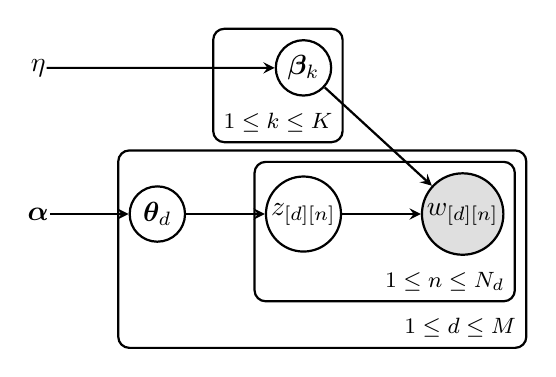
\begin{tikzpicture}[->, >=stealth, thick, scale=3.0]

    % Nodes

    \node[obs]                   (w)      {$w_{[d][n]}$} ; %
    \node[latent, left=of w]    (z)      {$z_{[d][n]}$} ; %
    \node[latent, left=of z]    (theta)  {$\bm{\theta}_d$}; %
    \node[const, left=of theta] (alpha) {$\bm{\alpha}$};

    \edge {z} {w}
    \edge {theta} {z}
    \edge {alpha} {theta}

    % More nodes
    \node[latent, above=of z] (beta)  {$\bm{\beta}_k$}; %
    \node[const]  (eta) at (alpha |- beta) {$\eta$}; %

    \edge {beta} {w}
    \edge {eta} {beta}

    \plate {plate1} { %
        (w)
        (z)
    } {$1 \leq n \leq N_d$}; %
    \plate {} { %
        (plate1) %
        (theta)
    } {$1 \leq d \leq M$} ; %
    \plate[align=left] {} { %
        (beta)
    } {$1 \leq k \leq K$} ; %

\end{tikzpicture}
\end{center}

\subsection{Intuition for LDA Model}

LDA can be used in the task of topic modeling, which is the task of extracting
word association patterns from a given corpus.  Under this use case, the
components of the LDA model take on some intuitive roles.

The $\bm{\beta}_{k}$ variable represents the $k$th distribution of word types;
this distribution is called a topic.  Suppose that there are $V$ word types.
Then the $v$th entry in $\bm{\beta}_{k}$ is the probability of the $v$th word
type occurring in the $k$th topic. The model tells us that there are $K$ topics.
Note that $K$ is arbitrarily chosen by the user.

The $\bm{\theta}_{d}$ variable represents the distribution of topics for the
$d$th document.  This means that a document is partially made up of topic 1,
partially of topic 2, and so forth.  The model tells us that there are $M$
documents in the corpus.

The $w_{[d][n]}$ variable represents the $n$th word of the $d$th document of the
corpus; it is the only variable in the model for which we have set values.  The
$z_{[d][n]}$ variable represents the topic assignment for the $n$th word of the
$d$th document.  The model tells us that there are $N_{d}$ word instances in the
$d$th document.

Finally, $\eta$ is a hyperparameter that encodes our bias for how word types
tend to be distributed in a topic, and $\bm{\alpha}$ is a hyperparameter that
encodes our bias for how topics are distributed in a document.  Thus, these
hyperparameters are arbitrarily chosen by the user.

\subsection{Joint Probability of LDA Model}

Based on the definition of the LDA model, we can see that the joint probability
of LDA is
\begin{align*}
    p(&\bm{\beta}_{1}, \ldots, \bm{\beta}_{K},\\
    & \bm{\theta}_{1}, \ldots, \bm{\theta}_{M},\\
    & z_{[1][1]}, z_{[1][2]}, \ldots, z_{[1][N_{1}]}, z_{[2][1]}, \ldots,
    z_{[M][1]}, \ldots, z_{[M][N_{M}]},\\
    & w_{[1][1]}, \ldots, w_{[M][N_{M}]}\\
    &\quad \mid \bm{\alpha}, \eta) =
    \left(\prod_{k=1}^{K}p(\bm{\beta}_{k} \mid \eta)\right)
    \left(\prod_{d=1}^{M}p(\bm{\theta}_{d} \mid \bm{\alpha})
    \prod_{n=1}^{N_{d}}p(z_{[d][n]} \mid \bm{\theta}_{d})
    p(w_{[d][n]} \mid z_{[d][n]}, \bm{\beta}_{1}, \ldots,
    \bm{\beta}_{K})\right).\numberthis\label{eq:jointp}
\end{align*}
Note that the parentheses around the product terms are rather arbitrary due to
the associativity of multiplication, but I find their placement clarifying.

We can also write out the log of the joint probability of LDA:
\begin{align*}
    &\log{p(\bm{\beta}_{1}, \ldots, \bm{\beta}_{K}, \bm{\theta}_{1}, \ldots,
    \bm{\theta}_{M}, z_{[1][1]}, \ldots, z_{[M][N_{M}]}, w_{[1][1]}, \ldots,
w_{[M][N_{M}]} \mid \bm{\alpha}, \eta)} = \\
    &\quad\quad\left(\sum_{k=1}^{K} \log{p(\bm{\beta}_{k} \mid
    \eta)}\right) + \\
    &\quad\quad\left(\sum_{d=1}^{M}\log{p(\bm{\theta}_{d} \mid
    \bm{\alpha})} + \sum_{n=1}^{N_{d}}\log{p(z_{[d][n]} \mid \bm{\theta}_{d}) +
    \log{p(w_{[d][n]} \mid z_{[d][n]}, \bm{\beta}_{1}, \ldots,
    \bm{\beta}_{K}})}\right)\numberthis\label{eq:logjointp},
\end{align*}
by applying the properties of logarithms.

\subsection{Posterior}

Although we know the assignments for our observed variables, $w_{[1][1]},
\ldots, w_{[M][N_{M}]}$, we would like to know the assignments for our latent
variables, $\bm{\beta}_{1}, \ldots, \bm{\beta}_{K}, \bm{\theta}_{1}, \ldots,
\bm{\theta}_{M}, z_{[1][1]}, \ldots, z_{[M][N_{M}]}$.  We can obtain the most
probable assignments for our latent variables, given that we know the setting of
our observed variables, by maximizing
\begin{equation}\label{eq:posterior}
    p(\bm{\beta}_{1}, \ldots, \bm{\beta}_{K}, \bm{\theta}_{1}, \ldots,
    \bm{\theta}_{M}, z_{[1][1]}, \ldots,
    z_{[M][N_{M}]} \mid w_{[1][1]}, \ldots, w_{[M][N_{M}]}, \bm{\alpha}, \eta).
\end{equation}
This turns out to be intractable because of the coupling between each
$\bm{\theta}_{d}$ and $\bm{\beta}_{1}, \ldots, \bm{\beta}_{K}$.\footnote{I admit
that I don't have a comprehensible explanation for why this is.}

\section{Approximate Model}

In order to apply the variational method to LDA, we need a model that
approximates LDA.  In this section, we spend time building up the approximate
model.

\subsection{Definition of Approximate Model}

\begin{equation}\label{eq:betadirlambda}
    \bm{\beta}_{k} \mid \bm{\lambda}_{d} \sim \text{Dir}(\bm{\lambda}_{d})
\end{equation}
\begin{equation}\label{eq:thetadirgamma}
    \bm{\theta}_{d} \mid \bm{\gamma}_{d} \sim \text{Dir}(\bm{\gamma}_{d})
\end{equation}
\begin{equation}\label{eq:zcatphi}
    z_{[d][n]} \mid \bm{\phi}_{[d][n]} \sim \text{Cat}(\bm{\phi}_{[d][n]})
\end{equation}

\begin{center}
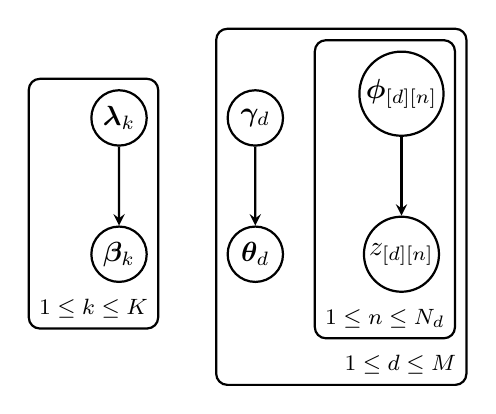
\begin{tikzpicture}[->, >=stealth, thick, scale=3.0]

    % Nodes

    \node[latent]    (z)      {$z_{[d][n]}$} ; %
    \node[latent, left=of z]    (theta)  {$\bm{\theta}_d$}; %
    \node[latent, left=of theta] (beta) {$\bm{\beta}_k$};

    % More nodes
    \node[latent, above=of z] (phi)  {$\bm{\phi}_{[d][n]}$}; %
    \node[latent, above=of theta]  (gamma) {$\bm{\gamma}_{d}$}; %
    \node[latent, above=of beta] (lambda) {$\bm{\lambda}_k$};

    \edge {phi} {z}
    \edge {gamma} {theta}
    \edge {lambda} {beta}

    \plate {plate1} { %
        (z)
        (phi)
    } {$1 \leq n \leq N_d$}; %
    \plate {} { %
        (plate1) %
        (theta)
        (gamma)
    } {$1 \leq d \leq M$} ; %
    \plate[align=left] {} { %
        (beta)
        (lambda)
    } {$1 \leq k \leq K$} ; %

\end{tikzpicture}
\end{center}

Note that we are re-using variables from LDA.  This is deliberate.  Since the
point of this model is to approximate LDA, and since we want to have the setting
of the latent variables that maximizes Eq.~\ref{eq:jointp}, we need some way to
represent those latent variables in this model.  Thus, the variables in this
model which share naming with variables in LDA correspond to their namesakes.

\subsection{Joint Probability of Approximate Model}

Note that in this model, $\bm{\lambda}_{k}$, $\bm{\gamma}_{d}$, and
$\bm{\phi}_{[d][n]}$ are really hyperparameters to $\bm{\beta}_{k}$,
$\bm{\theta}_{d}$, and $z_{[d][n]}$, respectively.  With this in mind, we can
claim the following to be the joint probability of this model:
\begin{align*}
    &\begin{aligned}q(&\bm{\beta}_{1}, \ldots, \bm{\beta}_{k}, \bm{\theta}_{1}, \ldots,
    \bm{\theta}_{M}, z_{[1][1]}, \ldots, z_{[M][N_{M}]} \mid \\*
    &\bm{\lambda}_{1},
    \ldots, \bm{\lambda}_{K}, \bm{\gamma}_{1}, \ldots, \bm{\gamma}_{M},
    \bm{\phi}_{[1][1]}, \ldots, \bm{\phi}_{[M][N_{M}]}) =
    \end{aligned}\\*
    &\quad\left(\prod_{k=1}^{K}q(\bm{\beta}_{k} \mid \bm{\lambda}_{k})\right)
    \left(\prod_{d=1}^{M}q(\bm{\theta}_{d} \mid \bm{\gamma}_{d})
    \prod_{n=1}^{N_{d}}q(z_{[d][n]} \mid \bm{\phi}_{[d][n]})\right).
    \numberthis\label{eq:jointq}
\end{align*}
Take special note that the distribution of this model is represented by $q$ (in
contrast to the distribution of LDA, which is represented by $p$).

We can even take the log of Eq.~\ref{eq:jointq}:
\begin{align*}
    &\begin{aligned}\log q(&\bm{\beta}_{1}, \ldots, \bm{\beta}_{k}, \bm{\theta}_{1}, \ldots,
    \bm{\theta}_{M}, z_{[1][1]}, \ldots, z_{[M][N_{M}]} \mid \\*
    &\bm{\lambda}_{1},
    \ldots, \bm{\lambda}_{K}, \bm{\gamma}_{1}, \ldots, \bm{\gamma}_{M},
    \bm{\phi}_{[1][1]}, \ldots, \bm{\phi}_{[M][N_{M}]}) =
    \end{aligned}\\*
    &\quad\left(\sum_{k=1}^{K}\log{q(\bm{\beta}_{k} \mid \bm{\lambda}_{k})}\right)
    + \left(\sum_{d=1}^{M}\log{q(\bm{\theta}_{d} \mid \bm{\gamma}_{d})}
    + \sum_{n=1}^{N_{d}}\log{q(z_{[d][n]} \mid \bm{\phi}_{[d][n]})}\right).
    \numberthis\label{eq:logjointq}
\end{align*}

As you may have noticed, all of the terms in our approximating model can be
fully factorized.\footnote{This is in contrast to Eq.~\ref{eq:jointp}, which has
the final product made up of two terms multiplied together (the multiplication
of these two terms causing the coupling between latent variables made LDA
intractable).}  Choosing to make our approximating distribution fully
factorizable is a strategy called the mean field assumption.  This is why the
variational approach explained in this document is called mean field variational
inference.

\section{Lower Bound for $\log{p(w_{[1][1]}, \ldots, w_{[M][N_{M}]} \mid
\bm{\alpha}, \eta)}$}

\subsection{Initial Algebra}

We now have enough information to begin contructing a lower bound, according to
the formula shown by Eq.~\ref{eq:lowerbound}.  Substituting $r$ with $p$ and $s$
with $q$, we get
\begin{align}
    &\log{p(w_{[1][1]}, \ldots, w_{[M][N_{M}]} \mid \bm{\alpha}, \eta)} \geq
    \nonumber\\
    &\quad\E_{q}[\log{p(\bm{\beta}_{1}, \ldots, \bm{\beta}_{K}, \bm{\theta}_{1},
    \ldots,
    \bm{\theta}_{M}, z_{[1][1]}, \ldots, z_{[M][N_{M}]}, w_{[1][1]}, \ldots,
    w_{[M][N_{M}]} \mid \bm{\alpha}, \eta))}] - \nonumber\\
    &\quad\quad\begin{aligned}
    \E_{q}[\log q(&\bm{\beta}_{1}, \ldots, \bm{\beta}_{k}, \bm{\theta}_{1}, \ldots,
    \bm{\theta}_{M}, z_{[1][1]}, \ldots, z_{[M][N_{M}]} \mid \\*
    &\bm{\lambda}_{1},
    \ldots, \bm{\lambda}_{K}, \bm{\gamma}_{1}, \ldots, \bm{\gamma}_{M},
    \bm{\phi}_{[1][1]}, \ldots, \bm{\phi}_{[M][N_{M}]})] =
    \end{aligned} \nonumber\\
    &\begin{aligned}
    &\begin{aligned}\E_{q}[&\left(\sum_{k=1}^{K} \log{p(\bm{\beta}_{k} \mid
    \eta)}\right) + \\*
    &\left(\sum_{d=1}^{M}\log{p(\bm{\theta}_{d} \mid
    \bm{\alpha})} + \sum_{n=1}^{N_{d}}\log{p(z_{[d][n]} \mid \bm{\theta}_{d})} +
    \log{p(w_{[d][n]} \mid z_{[d][n]}, \bm{\beta}_{1}, \ldots,
    \bm{\beta}_{K}})\right)] - \end{aligned} \\*
    &\quad\E_{q}[
    \left(\sum_{k=1}^{K}
    \log{q(\bm{\beta}_{k} \mid \bm{\lambda}_{k})}\right)
    + \left(\sum_{d=1}^{M}\log{q(\bm{\theta}_{d} \mid \bm{\gamma}_{d})}
    + \sum_{n=1}^{N_{d}}\log{q(z_{[d][n]} \mid
    \bm{\phi}_{[d][n]})}\right)] =
    \end{aligned}\label{eq:ldalb1} \\
    &\begin{aligned} & \left(\sum_{k=1}^{K} \E_{q} [\log p(\bm{\beta}_{k}
    \mid \eta)]\right) + \left( \sum_{d=1}^{M} \E_q[\log{p(\bm{\theta}_{d} \mid
    \bm{\alpha})}]\right) + \left( \sum_{d=1}^{M}\sum_{n=1}^{N_{d}}
    \E_q[\log{p(z_{[d][n]} \mid \bm{\theta}_{d})}]\right) + \\*
    &\quad\quad\left(
    \sum_{d=1}^{M} \sum_{n=1}^{N_{d}} \E_q[\log{p(w_{[d][n]} \mid z_{[d][n]},
    \bm{\beta}_{1}, \ldots, \bm{\beta}_{K})}] \right) - \\*
    &\quad\left( \sum_{k=1}^{K} \E_{q}[\log q(\bm{\beta}_{k} \mid
    \bm{\lambda}_{k})]\right) - \left(\sum_{d=1}^{M} \E_{q}[\log
    q(\bm{\theta}_{d} \mid \bm{\gamma}_{d})]\right) - \\*
    &\quad\quad\left( \sum_{d=1}^{M}
    \sum_{n=1}^{N_{d}} \E_{q}[\log q(z_{[d][n]} \mid \bm{\phi_{[d][n]}})]\right)
    = \end{aligned} \label{eq:ldalb2} \\
    &\begin{aligned}
    &\left(\sum_{k=1}^{K} \E_{q}[\log p(\bm{\beta}_{k} \mid \eta)] - \E_{q}[\log
    q(\bm{\beta}_{k} \mid \bm{\lambda}_{k})]\right) + \\*
    &\quad\left(\sum_{d=1}^{M} \E_{q}[\log p(\bm{\theta}_{d} \mid \bm{\alpha})]
    - \E_{q}[\log q(\bm{\theta}_{d} \mid \bm{\gamma}_{d})]\right) + \\*
    &\quad\left(\sum_{d=1}^{M}\sum_{n=1}^{N_{d}} \E_{q}[\log p(z_{[d][n]} \mid
    \bm{\theta}_{d})] + \E_{q}[\log p(w_{[d][n]} \mid z_{[d][n]}, \bm{\beta}_{1},
    \ldots, \bm{\beta}_{K})] - \E_{q}[\log q(z_{[d][n]} \mid
    \bm{\phi}_{[d][n]})]\right).
    \end{aligned}\label{eq:ldalb3}
\end{align}

Explanation:  Eq.~\ref{eq:ldalb1} applies both Eq.~\ref{eq:logjointp} and
Eq.~\ref{eq:logjointq}.  Eq.~\ref{eq:ldalb2} applies the $\E[a+b] = \E[a]+\E[b]$
property over all sums.  Eq.~\ref{eq:ldalb3} rearranges terms so that summations
are consolidated.

\subsection{Properties of Distributions}

To continue with Eq.~\ref{eq:ldalb3}, we need some probability density functions
(pdfs).  This subsection is devoted to showing what pdfs we need.

\subsubsection{Dirichlet Distributions}

Most of the information here comes from the Wikipedia article.

Let $\bm{x}$ be the random variable for a Dirichlet distribution $d$.  Note that
$\bm{x}$ is a vector of length $H$.  The hyperparameter for this distribution is
$\bm{\zeta}$, which is likewise a vector of length $H$.  Then its pdf is
\begin{equation}\label{eq:dirpdf}
    d(\bm{x} \mid \bm{\zeta}) =
    \frac{\Gamma (\sum_{h=1}^{H} \zeta_{h})}{\prod_{h=1}^{H} \Gamma (\zeta_{h})}
    \prod_{h=1}^{H}x_{h}^{\zeta_{h} - 1},
\end{equation}
where $\Gamma()$ is the gamma function.  Then the log of the pdf is
\begin{equation}\label{eq:logdirpdf}
    \log d(\bm{x} \mid \bm{\zeta}) =
    \log \Gamma(\sum_{h=1}^{H} \zeta_{h}) - \left(\sum_{h=1}^{H}
    \log \Gamma(\zeta_{h})\right) + \left(\sum_{h=1}^{H} (\zeta_{h} - 1) \log x_{h}
    \right).
\end{equation}

We will also want to know the expected value of the $\log$ of a certain value of
the random variable vector:
\begin{equation}\label{eq:expectedlogdir}
    \E [\log x_{h}] = \psi(\zeta_{h}) - \psi(\sum_{i=1}^{H} \zeta_{i}),
\end{equation}
where $\psi()$ is the digamma function (the derivative of $\log \Gamma()$).  For
a proof of this, see section 5.4.1 of \autocite{kb}.

\subsubsection{Symmetric Dirichlet Distributions}

A symmetric Dirichlet distribution is a Dirichlet distribution where all values
of the hyperparameter vector are equal to each other.  Thus, its pdf is
\begin{equation}\label{eq:symdirpdf}
    d(\bm{x} \mid \zeta) =
    \frac{\Gamma(H\zeta)}{(\Gamma(\zeta))^{H}}\prod_{h=1}^{H}x_{h}^{\zeta-1}.
\end{equation}
Therefore, the log pdf of a symmetric Dirichlet distribution is
\begin{equation}\label{eq:logsymdirpdf}
    \log d(\bm{x} \mid \zeta) =
    \log \Gamma(H\zeta) - H \log \Gamma(\zeta) + (\zeta - 1)
    (\sum_{h=1}^{H} \log x_{h}).
\end{equation}
Finally, the expected value of the $\log$ of a certain value of the random
variable vector is
\begin{equation}\label{eq:expectedlogsymdir}
    \E [\log x_{h}] = \psi(\zeta) - \psi(H\zeta).
\end{equation}

\subsubsection{Categorical Distributions}

Let $x$ be the random variable for a categorical distribution $c$.  Let the
vector $\bm{\xi}$ be its hyperparameter.  Then its pdf is
\begin{equation}\label{eq:catpdf}
    c(x \mid \bm{\xi}) = \xi_{x}.
\end{equation}
Hence, the log pdf of a categorical distribution is
\begin{equation}\label{eq:logcatpdf}
    \log c(x \mid \bm{\xi}) = \log \xi_{x}.
\end{equation}
The expected value of the log of a given random variable for a categorical
distribution is not as readily available as it was for a Dirichlet.  We will
come back to this problem in a little bit.

\subsection{A Little More Algebra}

Picking up from Eq.~\ref{eq:ldalb3}, where $V$ is the number of types in the
vocabulary,
\begin{align*}
    &\begin{aligned}
    &\left(\sum_{k=1}^{K} \E_{q}[\log p(\bm{\beta}_{k} \mid \eta)] - \E_{q}[\log
    q(\bm{\beta}_{k} \mid \bm{\lambda}_{k})]\right) + \\*
    &\quad\left(\sum_{d=1}^{M} \E_{q}[\log p(\bm{\theta}_{d} \mid \bm{\alpha})]
    - \E_{q}[\log q(\bm{\theta}_{d} \mid \bm{\gamma}_{d})]\right) + \\*
    &\quad\left(\sum_{d=1}^{M}\sum_{n=1}^{N_{d}} \E_{q}[\log p(z_{[d][n]} \mid
    \bm{\theta}_{d})] + \E_{q}[\log p(w_{[d][n]} \mid z_{[d][n]}, \bm{\beta}_{1},
    \ldots, \bm{\beta}_{K})] - \E_{q}[\log q(z_{[d][n]} \mid
    \bm{\phi}_{[d][n]})]\right) =
    \end{aligned}\\
    &\begin{aligned}
    &\begin{aligned}\left(\sum_{k=1}^{K} \right. &\E_{q}[ \log \Gamma(V\eta) -
    V \log \Gamma(\eta) + (\eta - 1) (\sum_{v=1}^{V} \log \beta_{[k][v]}) ] -
    \\*
    &\left. \E_{q} [ \log
    \Gamma(\sum_{v=1}^{V} \lambda_{[k][v]}) - \left(\sum_{v=1}^{V} \log
    \Gamma(\lambda_{[k][v]})\right) + \left(\sum_{v=1}^{V} (\lambda_{[k][v]} - 1) \log
    \beta_{[k][v]}\right)]\right) +\end{aligned} \\*
    &\quad\begin{aligned}\left(\sum_{d=1}^{M}\right. &\left.\E_{q}[\log \Gamma
    (\sum_{k=1}^{K}
    \alpha_{k}) - \left(\sum_{k=1}^{K}\log \Gamma(\alpha_{k})\right) +
    \left(\sum_{k=1}^{K}(\alpha_{k} - 1)\log \theta_{[d][k]}\right)]\right. -
    \\*
    &\left.\E_{q}[\log \Gamma(\sum_{k=1}^{K} \gamma_{[d][k]}) - \left(\sum_{k=1}^{K}
    \log \Gamma(\gamma_{[d][k]})\right) + \left(\sum_{k=1}^{K} (\gamma_{[d][k]} - 1)
    \log \theta_{[d][k]}\right)]\right) +
    \end{aligned}\\*
    &\quad\begin{aligned}
    \left(\sum_{d=1}^{M}\sum_{n=1}^{N_{d}} \E_{q}[\log \theta_{[d][z_{[d][n]}]}]
    + \E_{q}[\log \beta_{[z_{[d][n]}][w_{[d][n]}]}] -
    \E_{q}[\log \phi_{[d][n][z_{[d][n]}]}]\right) =
    \end{aligned}
    \end{aligned}\numberthis\label{eq:lbpdf1}\\
    &\begin{aligned}
    &\begin{aligned}\left(\sum_{k=1}^{K} \right. &\E_{q}[ \log \Gamma(V\eta)]
    - \E_{q}[V \log \Gamma(\eta)] + \E_{q}[(\eta - 1) (\sum_{v=1}^{V} \log
    \beta_{[k][v]}) ] - \\*
    &\left. \E_{q} [ \log \Gamma(\sum_{v=1}^{V} \lambda_{[k][v]}) ] +
    \E_{q}[ \left(\sum_{v=1}^{V} \log \Gamma(\lambda_{[k][v]})\right) ] -
    \E_{q}[ \left(\sum_{v=1}^{V} (\lambda_{[k][v]} - 1) \log
    \beta_{[k][v]}\right)]\right) +\end{aligned} \\*
    &\quad\begin{aligned}\left(\sum_{d=1}^{M}\right. &\left.\E_{q}[\log \Gamma
    (\sum_{k=1}^{K} \alpha_{k})] -
    \E_{q}[\left(\sum_{k=1}^{K}\log \Gamma(\alpha_{k})\right)] +
    \E_{q}[\left(\sum_{k=1}^{K}(\alpha_{k} - 1)\log \theta_{[d][k]}\right)]
    \right. - \\*
    &\left.\E_{q}[\log \Gamma(\sum_{k=1}^{K} \gamma_{[d][k]})] +
    \E_{q}[\left(\sum_{k=1}^{K} \log \Gamma(\gamma_{[d][k]})\right)] -
    \E_{q}[\left(\sum_{k=1}^{K} (\gamma_{[d][k]} - 1) \log \theta_{[d][k]}
    \right)]\right) +
    \end{aligned}\\*
    &\quad\begin{aligned}
    \left(\sum_{d=1}^{M}\sum_{n=1}^{N_{d}} \E_{q}[\log \theta_{[d][z_{[d][n]}]}]
    + \E_{q}[\log \beta_{[z_{[d][n]}][w_{[d][n]}]}] -
    \E_{q}[\log \phi_{[d][n][z_{[d][n]}]}]\right) =
    \end{aligned}
    \end{aligned}\numberthis\label{eq:lbpdf2}\\
    &\begin{aligned}
    &\begin{aligned}\left(\sum_{k=1}^{K} \right. &\E_{q}[ \log \Gamma(V\eta)]
    - \E_{q}[V \log \Gamma(\eta)] + (\eta - 1) \left(\sum_{v=1}^{V}\E_{q}[ \log
    \beta_{[k][v]} ]\right) - \\*
    &\left. \E_{q} [ \log \Gamma(\sum_{v=1}^{V} \lambda_{[k][v]}) ] +
    \left(\sum_{v=1}^{V} \E_{q}[ \log \Gamma(\lambda_{[k][v]}) ]\right) -
    \left(\sum_{v=1}^{V} \E_{q}[ (\lambda_{[k][v]} - 1) \log
    \beta_{[k][v]}]\right)\right) +\end{aligned} \\*
    &\quad\begin{aligned}\left(\sum_{d=1}^{M}\right. &\left.\E_{q}[\log \Gamma
    (\sum_{k=1}^{K} \alpha_{k})] -
    \left(\sum_{k=1}^{K}\E_{q}[\log \Gamma(\alpha_{k})]\right) +
    \left(\sum_{k=1}^{K}\E_{q}[(\alpha_{k} - 1)\log \theta_{[d][k]}]\right)
    \right. - \\*
    &\left.\E_{q}[\log \Gamma(\sum_{k=1}^{K} \gamma_{[d][k]})] +
    \left(\sum_{k=1}^{K} \E_{q}[\log \Gamma(\gamma_{[d][k]})]\right) -
    \left(\sum_{k=1}^{K} \E_{q}[(\gamma_{[d][k]} - 1) \log \theta_{[d][k]}
    ]\right)\right) +
    \end{aligned}\\*
    &\quad\begin{aligned}
    \left(\sum_{d=1}^{M}\sum_{n=1}^{N_{d}} \E_{q}[\log \theta_{[d][z_{[d][n]}]}]
    + \E_{q}[\log \beta_{[z_{[d][n]}][w_{[d][n]}]}] -
    \E_{q}[\log \phi_{[d][n][z_{[d][n]}]}]\right) =
    \end{aligned}
    \end{aligned}\numberthis\label{eq:lbpdf3}\\
    &\begin{aligned}
    &\begin{aligned}\left(\sum_{k=1}^{K} \right. &\log \Gamma(V\eta)
    - V \log \Gamma(\eta) + (\eta - 1) \left(\sum_{v=1}^{V}\E_{q}[ \log
    \beta_{[k][v]} ]\right) - \\*
    &\left. \log \Gamma(\sum_{v=1}^{V} \lambda_{[k][v]}) +
    \left(\sum_{v=1}^{V} \log \Gamma(\lambda_{[k][v]}) \right) -
    \left(\sum_{v=1}^{V} (\lambda_{[k][v]} - 1) \E_{q}[ \log
    \beta_{[k][v]}]\right)\right) +\end{aligned} \\*
    &\quad\begin{aligned}\left(\sum_{d=1}^{M}\right. &\left.\log \Gamma
    (\sum_{k=1}^{K} \alpha_{k}) -
    \left(\sum_{k=1}^{K}\log \Gamma(\alpha_{k})\right) +
    \left(\sum_{k=1}^{K}(\alpha_{k} - 1)\E_{q}[\log \theta_{[d][k]}]\right)
    \right. - \\*
    &\left.\log \Gamma(\sum_{k=1}^{K} \gamma_{[d][k]}) +
    \left(\sum_{k=1}^{K} \log \Gamma(\gamma_{[d][k]})\right) -
    \left(\sum_{k=1}^{K} (\gamma_{[d][k]} - 1) \E_{q}[\log \theta_{[d][k]}
    ]\right)\right) +
    \end{aligned}\\*
    &\quad\begin{aligned}
    \left(\sum_{d=1}^{M}\sum_{n=1}^{N_{d}} \E_{q}[\log \theta_{[d][z_{[d][n]}]}]
    + \E_{q}[\log \beta_{[z_{[d][n]}][w_{[d][n]}]}] -
    \E_{q}[\log \phi_{[d][n][z_{[d][n]}]}]\right) =
    \end{aligned}
    \end{aligned}\numberthis\label{eq:lbpdf4}\\
    &\begin{aligned}
    &\begin{aligned}\left(\sum_{k=1}^{K} \right. &\log \Gamma(V\eta)
    - V \log \Gamma(\eta) + (\eta - 1) \left(\sum_{v=1}^{V}
    (\psi(\lambda_{[k][v]}) - \psi(\sum_{v'=1}^{V} \lambda_{[k][v']}))\right) -
    \\*
    &\left. \log \Gamma(\sum_{v=1}^{V} \lambda_{[k][v]}) +
    \left(\sum_{v=1}^{V} \log \Gamma(\lambda_{[k][v]}) \right) -
    \left(\sum_{v=1}^{V} (\lambda_{[k][v]} - 1)
    (\psi(\lambda_{[k][v]}) - \psi(\sum_{v'=1}^{V} \lambda_{[k][v']}))
    \right)\right) +\end{aligned} \\*
    &\quad\begin{aligned}\left(\sum_{d=1}^{M}\right. &\left.\log \Gamma
    (\sum_{k=1}^{K} \alpha_{k}) -
    \left(\sum_{k=1}^{K}\log \Gamma(\alpha_{k})\right) +
    \left(\sum_{k=1}^{K}(\alpha_{k} - 1)
    (\psi(\gamma_{[d][v]}) - \psi(\sum_{k'=1}^{K} \gamma_{[d][k']}))
    \right)
    \right. - \\*
    &\left.\log \Gamma(\sum_{k=1}^{K} \gamma_{[d][k]}) +
    \left(\sum_{k=1}^{K} \log \Gamma(\gamma_{[d][k]})\right) -
    \left(\sum_{k=1}^{K} (\gamma_{[d][k]} - 1)
    (\psi(\gamma_{[d][v]}) - \psi(\sum_{k'=1}^{K} \gamma_{[d][k']}))
    \right)\right) +
    \end{aligned}\\*
    &\quad\begin{aligned}
    \left(\sum_{d=1}^{M}\sum_{n=1}^{N_{d}} \E_{q}[\log \theta_{[d][z_{[d][n]}]}]
    + \E_{q}[\log \beta_{[z_{[d][n]}][w_{[d][n]}]}] -
    \E_{q}[\log \phi_{[d][n][z_{[d][n]}]}]\right).
    \end{aligned}
    \end{aligned}\numberthis\label{eq:lbpdf5}\\
\end{align*}
Explanation:  Eq.~\ref{eq:lbpdf1} substitutes log probabilities with log pdfs.
We know which log pdfs to use thanks to the definitions of each of the
probabilities (Eqs.~\ref{eq:betadireta}, \ref{eq:thetadiralpha},
\ref{eq:zcattheta}, \ref{eq:wcatz}, \ref{eq:betadirlambda},
\ref{eq:thetadirgamma}, and \ref{eq:zcatphi}).  Eq.~\ref{eq:lbpdf2} applies the
rule $\E[a+b] = \E[a]+\E[b]$.  Eq.~\ref{eq:lbpdf3} applies the same rule again
(this time, pushing the expectation into the summations).  Noting that none of
the hyperparameters $\eta$, $\lambda_{[k][v]}, \alpha_{k},$ and
$\gamma_{[d][k]}$ vary in $q$, the expected value of these terms is simply those
terms; Eq.~\ref{eq:lbpdf4} applies this.  Of course, $\phi_{[d][n][k]}$ is also
a hyperparameter, but that term never shows up by itself:
$\phi_{[d][n][z_{[d][n]}]}$ relies on $z_{[d][n]}$, which does vary in $q$,
which is why that expected value is not simply the expression within the
brackets.  In Eq.~\ref{eq:lbpdf5}, we apply
Eqs.~\ref{eq:expectedlogdir}~and~\ref{eq:expectedlogsymdir}.

\subsection{Expected Values of the Log of Categorical Distributions}

We pause from our algebra to consider what expression ought to replace the
expected values of the log categoricals.

\subsubsection{$\E_{q}[\log \theta_{[d][z_{[d][n]}]}]$}

Let's begin with $\E_{q}[\log \theta_{[d][z_{[d][n]}]}]$.  Expanding the
expectation according to its definition,
\begin{align*}
    &\E_{q}[\log \theta_{[d][z_{[d][n]}]}] = \\
    &\quad\int \cdots \int
    \sum_{z_{[1][1]}=1}^{K} \cdots \sum_{z_{[M][N_{M}]}=1}^{K} \\
    &\quad\quad\begin{aligned} q(&\bm{\beta}_{1}, \ldots, \bm{\beta}_{K},
    \bm{\theta}_{1}, \ldots \bm{\theta}_{M}, z_{[1][1]}, \ldots, z_{[M][N_{M}]}
    \mid \\*
    & \bm{\lambda}_{1}, \ldots, \bm{\lambda}_{K}, \bm{\gamma}_{1}, \ldots,
    \bm{\gamma}_{M}, \bm{\phi}_{[1][1]}, \ldots, \bm{\phi}_{[M][N_{M}]})\log
    \theta_{[d][z_{[d][n]}]}
    \end{aligned} \\
    &\quad d\bm{\beta}_{1}\cdots d\bm{\beta}_{K}d\bm{\theta}_{1}\cdots
    d\bm{\theta}_{M}.
    \numberthis
\end{align*}
Note that the expectation of some random variable $x$ with respect to some
distribution $s$ is the sum of all possible settings for each free variable in
$s$ multiplied by $x$ at those settings.  Of course, this means that when the
free variable can take on any real value, the sum over all possible settings of
that variable becomes an integral.

We can expand $q$ according to Eq.~\ref{eq:jointq}:
\begin{align*}
    &\int \cdots \int
    \sum_{z_{[1][1]}=1}^{K} \cdots \sum_{z_{[M][N_{M}]}=1}^{K} \\
    &\quad\quad\begin{aligned} q(&\bm{\beta}_{1}, \ldots, \bm{\beta}_{K},
    \bm{\theta}_{1}, \ldots \bm{\theta}_{M}, z_{[1][1]}, \ldots, z_{[M][N_{M}]}
    \mid \\*
    & \bm{\lambda}_{1}, \ldots, \bm{\lambda}_{K}, \bm{\gamma}_{1}, \ldots,
    \bm{\gamma}_{M}, \bm{\phi}_{[1][1]}, \ldots, \bm{\phi}_{[M][N_{M}]})\log
    \theta_{[d][z_{[d][n]}]}
    \end{aligned} \\
    &\quad d\bm{\beta}_{1}\cdots d\bm{\beta}_{K}d\bm{\theta}_{1}\cdots
    d\bm{\theta}_{M} = \numberthis \\
    \numberthis
    &\int \cdots \int
    \sum_{z_{[1][1]}=1}^{K} \cdots \sum_{z_{[M][N_{M}]}=1}^{K} \\
    &\quad\quad\left(\prod_{k'=1}^{K} q(\bm{\beta}_{k'} \mid
    \bm{\lambda}_{k'})\right)
    \left(\prod_{d'=1}^{M}q(\bm{\theta}_{d'} \mid \bm{\gamma}_{d'})
    \prod_{n'=1}^{N_{d}}q(z_{[d'][n']} \mid \bm{\phi}_{[d'][n']})\right)
    \log \theta_{[d][z_{[d][n]}]}\\
    &\quad d\bm{\beta}_{1}\cdots d\bm{\beta}_{K}d\bm{\theta}_{1}\cdots
    d\bm{\theta}_{M}. \numberthis
\end{align*}

Looking at the expression within the integrations and summations, we can see
that nearly all of the terms factor out nicely.  In other words, no matter how
many times we add up $q(\bm{\beta}_{k'} \mid
\bm{\lambda}_{k'})\log\theta_{[d][z_{[d][n]}]}$ while changing the value of
$z_{[d][n]}$ and holding $\bm{\beta}_{k'}$ fixed, $q(\bm{\beta}_{k'} \mid
\bm{\lambda}_{k'})$ will be the same value.  Thus, we can safely factor
$q(\bm{\beta}_{k'} \mid \bm{\lambda}_{k'})$ out from the summation over all
possible values of $z_{[d][n]}$.  Another way to say this:
\begin{equation}
    \sum_{z_{[d][n]}=1}^{K} q(\bm{\beta}_{k'} \mid \bm{\lambda}_{k'}) \log
    \theta_{[d][z_{[d][n]}]} = q(\bm{\beta}_{k'} \mid \bm{\lambda}_{k'})
    \sum_{z_{[d][n]}=1}^{K} \log \theta_{[d][z_{[d][n]}]}.
\end{equation}
This same logic can be applied to all variables not present in the expression
$\log \theta_{[d][z_{[d][n]}]}$:
\begin{align*}
    &\int \cdots \int
    \sum_{z_{[1][1]}=1}^{K} \cdots \sum_{z_{[M][N_{M}]}=1}^{K} \\*
    &\quad\quad\left(\prod_{k'=1}^{K} q(\bm{\beta}_{k'} \mid
    \bm{\lambda}_{k'})\right) \left(\prod_{d'=1}^{M}q(\bm{\theta}_{d'} \mid \bm{\gamma}_{d'})
    \prod_{n'=1}^{N_{d}}q(z_{[d'][n']} \mid \bm{\phi}_{[d'][n']})\right)
    \log \theta_{[d][z_{[d][n]}]}\\*
    &\quad d\bm{\beta}_{1}\cdots d\bm{\beta}_{K}d\bm{\theta}_{1}\cdots
    d\bm{\theta}_{M} = \numberthis \\
    &\int \cdots \int
    \sum_{z_{[1][1]}=1}^{K} \cdots \sum_{z_{[d][n-1]}=1}^{K}
    \sum_{z_{[d][n+1]=1}}^{K} \cdots \sum_{z_{[M][N_{M}]}=1}^{K} \\*
    &\quad\quad\left(\prod_{k'=1}^{K} q(\bm{\beta}_{k'} \mid
    \bm{\lambda}_{k'})\right)
    \left(\prod_{d'=1, d'\neq d}^{M}q(\bm{\theta}_{d'} \mid \bm{\gamma}_{d'})\right)
    \left(\prod_{d'=1}^{M}\prod_{n'=1, n'\neq n}^{N_{d}}q(z_{[d'][n']} \mid
    \bm{\phi}_{[d'][n']})\right) \\*
    &\quad\quad\quad\sum_{z_{[d][n]=1}}^{K} q(\bm{\theta}_{d} \mid \bm{\gamma}_{d}) q(z_{[d][n]}
    \mid \bm{\phi}_{[d][n]})\log \theta_{[d][z_{[d][n]}]}\\*
    &\quad d\bm{\beta}_{1}\cdots d\bm{\beta}_{K}d\bm{\theta}_{1}\cdots
    d\bm{\theta}_{M} = \numberthis \\
    &\int \cdots \int \left(\prod_{k'=1}^{K} q(\bm{\beta}_{k'} \mid
    \bm{\lambda}_{k'})\right)
    \left(\prod_{d'=1, d'\neq d}^{M}q(\bm{\theta}_{d'} \mid \bm{\gamma}_{d'})\right)
    \sum_{z_{[1][1]}=1}^{K} \cdots \sum_{z_{[d][n-1]}=1}^{K}
    \sum_{z_{[d][n+1]=1}}^{K} \cdots \sum_{z_{[M][N_{M}]}=1}^{K} \\*
    &\quad\quad \left(\prod_{d'=1}^{M}\prod_{n'=1, n'\neq n}^{N_{d}}
    q(z_{[d'][n']} \mid
    \bm{\phi}_{[d'][n']})\right) \\*
    &\quad\quad\quad\sum_{z_{[d][n]=1}}^{K} q(\bm{\theta}_{d} \mid \bm{\gamma}_{d}) q(z_{[d][n]}
    \mid \bm{\phi}_{[d][n]})\log \theta_{[d][z_{[d][n]}]}\\*
    &\quad d\bm{\beta}_{1}\cdots d\bm{\beta}_{K}d\bm{\theta}_{1}\cdots
    d\bm{\theta}_{M}.
    \numberthis
\end{align*}

We took the liberty of factoring a few more terms than mentioned in the earlier
explanation.  This helps us see more clearly that we are taking the integral of
a probability distribution over all possible settings of that probability
distribution.  Of course, by the axioms of probability, that integral must be
equal to one.  Repeatedly applying this process lets us eliminate many terms:
\begin{align*}
    &\int \cdots \int \left(\prod_{k'=1}^{K} q(\bm{\beta}_{k'} \mid
    \bm{\lambda}_{k'})\right)
    \left(\prod_{d'=1, d'\neq d}^{M}q(\bm{\theta}_{d'} \mid \bm{\gamma}_{d'})\right)
    \sum_{z_{[1][1]}=1}^{K} \cdots \sum_{z_{[d][n-1]}=1}^{K}
    \sum_{z_{[d][n+1]=1}}^{K} \cdots \sum_{z_{[M][N_{M}]}=1}^{K} \\*
    &\quad\quad \left(\prod_{d'=1}^{M}\prod_{n'=1, n'\neq n}^{N_{d}}
    q(z_{[d'][n']} \mid
    \bm{\phi}_{[d'][n']})\right) \\*
    &\quad\quad\quad\sum_{z_{[d][n]=1}}^{K} q(\bm{\theta}_{d} \mid \bm{\gamma}_{d}) q(z_{[d][n]}
    \mid \bm{\phi}_{[d][n]})\log \theta_{[d][z_{[d][n]}]}\\*
    &\quad d\bm{\beta}_{1}\cdots d\bm{\beta}_{K}d\bm{\theta}_{1}\cdots
    d\bm{\theta}_{M} = \numberthis \\
    &\int \cdots \int q(\bm{\beta}_{1} \mid \bm{\lambda}_{1})
    \left(\left(\prod_{k'=2}^{K} q(\bm{\beta}_{k'} \mid \bm{\lambda}_{k'})\right)
    \left(\prod_{d'=1, d'\neq d}^{M}q(\bm{\theta}_{d'} \mid \bm{\gamma}_{d'})\right)
    \sum_{z_{[1][1]}=1}^{K} \cdots \sum_{z_{[d][n-1]}=1}^{K}
    \sum_{z_{[d][n+1]=1}}^{K} \cdots \sum_{z_{[M][N_{M}]}=1}^{K} \right.\\*
    &\quad\quad \left(\prod_{d'=1}^{M}\prod_{n'=1, n'\neq n}^{N_{d}}
    q(z_{[d'][n']} \mid
    \bm{\phi}_{[d'][n']})\right) \\*
    &\left.\quad\quad\quad\sum_{z_{[d][n]=1}}^{K}
    q(\bm{\theta}_{d} \mid \bm{\gamma}_{d}) q(z_{[d][n]}
    \mid \bm{\phi}_{[d][n]})\log \theta_{[d][z_{[d][n]}]}\right)\\*
    &\quad d\bm{\beta}_{1}\cdots d\bm{\beta}_{K}d\bm{\theta}_{1}\cdots
    d\bm{\theta}_{M} = \numberthis \\
    &\int \cdots \int
    \left(\left(\prod_{k'=2}^{K} q(\bm{\beta}_{k'} \mid \bm{\lambda}_{k'})\right)
    \left(\prod_{d'=1, d'\neq d}^{M}q(\bm{\theta}_{d'} \mid \bm{\gamma}_{d'})\right)
    \sum_{z_{[1][1]}=1}^{K} \cdots \sum_{z_{[d][n-1]}=1}^{K}
    \sum_{z_{[d][n+1]=1}}^{K} \cdots \sum_{z_{[M][N_{M}]}=1}^{K} \right.\\*
    &\quad\quad \left(\prod_{d'=1}^{M}\prod_{n'=1, n'\neq n}^{N_{d}}
    q(z_{[d'][n']} \mid
    \bm{\phi}_{[d'][n']})\right) \\*
    &\left.\quad\quad\quad\sum_{z_{[d][n]=1}}^{K}
    q(\bm{\theta}_{d} \mid \bm{\gamma}_{d}) q(z_{[d][n]}
    \mid \bm{\phi}_{[d][n]})\log \theta_{[d][z_{[d][n]}]}\right)
    q(\bm{\beta}_{1} \mid \bm{\lambda}_{1})\\*
    &\quad d\bm{\beta}_{1}\cdots d\bm{\beta}_{K}d\bm{\theta}_{1}\cdots
    d\bm{\theta}_{M} = \numberthis \\
    &\int \cdots \int
    \left(\left(\prod_{k'=2}^{K} q(\bm{\beta}_{k'} \mid \bm{\lambda}_{k'})\right)
    \left(\prod_{d'=1, d'\neq d}^{M}q(\bm{\theta}_{d'} \mid \bm{\gamma}_{d'})\right)
    \sum_{z_{[1][1]}=1}^{K} \cdots \sum_{z_{[d][n-1]}=1}^{K}
    \sum_{z_{[d][n+1]=1}}^{K} \cdots \sum_{z_{[M][N_{M}]}=1}^{K} \right.\\*
    &\quad\quad \left(\prod_{d'=1}^{M}\prod_{n'=1, n'\neq n}^{N_{d}}
    q(z_{[d'][n']} \mid
    \bm{\phi}_{[d'][n']})\right) \\*
    &\left.\quad\quad\quad\sum_{z_{[d][n]=1}}^{K}
    q(\bm{\theta}_{d} \mid \bm{\gamma}_{d}) q(z_{[d][n]}
    \mid \bm{\phi}_{[d][n]})\log \theta_{[d][z_{[d][n]}]}\right)
    \int q(\bm{\beta}_{1} \mid \bm{\lambda}_{1})\\*
    &\quad d\bm{\beta}_{1}\cdots d\bm{\beta}_{K}d\bm{\theta}_{1}\cdots
    d\bm{\theta}_{M} = \numberthis \\
    &\int \cdots \int
    \left(\left(\prod_{k'=2}^{K} q(\bm{\beta}_{k'} \mid \bm{\lambda}_{k'})\right)
    \left(\prod_{d'=1, d'\neq d}^{M}q(\bm{\theta}_{d'} \mid \bm{\gamma}_{d'})\right)
    \sum_{z_{[1][1]}=1}^{K} \cdots \sum_{z_{[d][n-1]}=1}^{K}
    \sum_{z_{[d][n+1]=1}}^{K} \cdots \sum_{z_{[M][N_{M}]}=1}^{K} \right.\\*
    &\quad\quad \left(\prod_{d'=1}^{M}\prod_{n'=1, n'\neq n}^{N_{d}}
    q(z_{[d'][n']} \mid
    \bm{\phi}_{[d'][n']})\right) \\*
    &\left.\quad\quad\quad\sum_{z_{[d][n]=1}}^{K}
    q(\bm{\theta}_{d} \mid \bm{\gamma}_{d}) q(z_{[d][n]}
    \mid \bm{\phi}_{[d][n]})\log \theta_{[d][z_{[d][n]}]}\right)
    \cdot 1\\*
    &\quad d\bm{\beta}_{2}\cdots d\bm{\beta}_{K}d\bm{\theta}_{1}\cdots
    d\bm{\theta}_{M} = \numberthis \\
    &\int \cdots \int
    \left(\left(\prod_{k'=2}^{K} q(\bm{\beta}_{k'} \mid \bm{\lambda}_{k'})\right)
    \left(\prod_{d'=1, d'\neq d}^{M}q(\bm{\theta}_{d'} \mid \bm{\gamma}_{d'})\right)
    \sum_{z_{[1][1]}=1}^{K} \cdots \sum_{z_{[d][n-1]}=1}^{K}
    \sum_{z_{[d][n+1]=1}}^{K} \cdots \sum_{z_{[M][N_{M}]}=1}^{K} \right.\\*
    &\quad\quad \left(\prod_{d'=1}^{M}\prod_{n'=1, n'\neq n}^{N_{d}}
    q(z_{[d'][n']} \mid
    \bm{\phi}_{[d'][n']})\right) \\*
    &\left.\quad\quad\quad\sum_{z_{[d][n]=1}}^{K}
    q(\bm{\theta}_{d} \mid \bm{\gamma}_{d}) q(z_{[d][n]}
    \mid \bm{\phi}_{[d][n]})\log \theta_{[d][z_{[d][n]}]}\right)\\*
    &\quad d\bm{\beta}_{2}\cdots d\bm{\beta}_{K}d\bm{\theta}_{1}\cdots
    d\bm{\theta}_{M} = \numberthis \\
    &\intertext{\begin{equation*} \vdots \end{equation*}}\\
    &\int
    \sum_{z_{[1][1]}=1}^{K} \cdots \sum_{z_{[d][n-1]}=1}^{K}
    \sum_{z_{[d][n+1]=1}}^{K} \cdots \sum_{z_{[M][N_{M}]}=1}^{K}\\*
    &\quad\quad \left(\prod_{d'=1}^{M}\prod_{n'=1, n'\neq n}^{N_{d}}
    q(z_{[d'][n']} \mid
    \bm{\phi}_{[d'][n']})\right) \\*
    &\quad\quad\quad\sum_{z_{[d][n]=1}}^{K}
    q(\bm{\theta}_{d} \mid \bm{\gamma}_{d}) q(z_{[d][n]}
    \mid \bm{\phi}_{[d][n]})\log \theta_{[d][z_{[d][n]}]}\\*
    &\quad d\bm{\theta}_{d}.
    \numberthis
\end{align*}
The same strategy applies to the summations:
\begin{align*}
    &\int
    \sum_{z_{[1][1]}=1}^{K} \cdots \sum_{z_{[d][n-1]}=1}^{K}
    \sum_{z_{[d][n+1]=1}}^{K} \cdots \sum_{z_{[M][N_{M}]}=1}^{K}\\*
    &\quad\quad \left(\prod_{d'=1}^{M}\prod_{n'=1, n'\neq n}^{N_{d}}
    q(z_{[d'][n']} \mid
    \bm{\phi}_{[d'][n']})\right) \\*
    &\quad\quad\quad\sum_{z_{[d][n]=1}}^{K}
    q(\bm{\theta}_{d} \mid \bm{\gamma}_{d}) q(z_{[d][n]}
    \mid \bm{\phi}_{[d][n]})\log \theta_{[d][z_{[d][n]}]}\\*
    &\quad d\bm{\theta}_{d} = \numberthis \\
    &\int
    \sum_{z_{[1][1]}=1}^{K} \cdots \sum_{z_{[d][n-1]}=1}^{K}
    \sum_{z_{[d][n+1]=1}}^{K} \cdots \sum_{z_{[M][N_{M}]}=1}^{K}\\*
    &\quad\quad\quad\left(\sum_{z_{[d][n]=1}}^{K}
    q(\bm{\theta}_{d} \mid \bm{\gamma}_{d}) q(z_{[d][n]}
    \mid \bm{\phi}_{[d][n]})\log \theta_{[d][z_{[d][n]}]}\right)\\*
    &\quad\quad \left(\prod_{d'=1}^{M}\prod_{n'=1, n'\neq n}^{N_{d}}
    q(z_{[d'][n']} \mid
    \bm{\phi}_{[d'][n']})\right) \\*
    &\quad d\bm{\theta}_{d} = \numberthis \\
    &\int
    \left(\sum_{z_{[d][n]=1}}^{K}
    q(\bm{\theta}_{d} \mid \bm{\gamma}_{d}) q(z_{[d][n]}
    \mid \bm{\phi}_{[d][n]})\log \theta_{[d][z_{[d][n]}]}\right)\\*
    &\quad\sum_{z_{[1][1]}=1}^{K} \cdots \sum_{z_{[d][n-1]}=1}^{K}
    \sum_{z_{[d][n+1]=1}}^{K} \cdots \sum_{z_{[M][N_{M}]}=1}^{K}\\*
    &\quad\quad \left(\prod_{d'=1}^{M}\prod_{n'=1, n'\neq n}^{N_{d}}
    q(z_{[d'][n']} \mid
    \bm{\phi}_{[d'][n']})\right) \\*
    &\quad d\bm{\theta}_{d} = \numberthis \\
    &\int
    \left(\sum_{z_{[d][n]=1}}^{K}
    q(\bm{\theta}_{d} \mid \bm{\gamma}_{d}) q(z_{[d][n]}
    \mid \bm{\phi}_{[d][n]})\log \theta_{[d][z_{[d][n]}]}\right)\\*
    &\quad\sum_{z_{[1][1]}=1}^{K} \cdots \sum_{z_{[d][n-1]}=1}^{K}
    \sum_{z_{[d][n+1]=1}}^{K} \cdots \sum_{z_{[M][N_{M}]}=1}^{K}\\*
    &\quad\quad \left(\prod_{d'=1}^{M-1}\prod_{n'=1, n'\neq n}^{N_{d}}
    q(z_{[d'][n']} \mid \bm{\phi}_{[d'][n']})\right)
    \left(\prod_{n'=1}^{N_{M}-1}q(z_{[M][n']} \mid \bm{\phi}_{[M][n']})\right)
    q(z_{[M][N_{M}]} \mid \bm{\phi}_{[M][N_{M}]}) \\*
    &\quad d\bm{\theta}_{d} = \numberthis \\
    &\int
    \left(\sum_{z_{[d][n]=1}}^{K}
    q(\bm{\theta}_{d} \mid \bm{\gamma}_{d}) q(z_{[d][n]}
    \mid \bm{\phi}_{[d][n]})\log \theta_{[d][z_{[d][n]}]}\right)\\*
    &\quad\sum_{z_{[1][1]}=1}^{K} \cdots \sum_{z_{[d][n-1]}=1}^{K}
    \sum_{z_{[d][n+1]=1}}^{K} \cdots \sum_{z_{[M][N_{M}-1]}=1}^{K}\\*
    &\quad\quad \left(\prod_{d'=1}^{M-1}\prod_{n'=1, n'\neq n}^{N_{d}}
    q(z_{[d'][n']} \mid \bm{\phi}_{[d'][n']})\right)
    \left(\prod_{n'=1}^{N_{M}-1}q(z_{[M][n']} \mid \bm{\phi}_{[M][n']})\right)
    \sum_{z_{[M][N_{M}]}=1}^{K}
    q(z_{[M][N_{M}]} \mid \bm{\phi}_{[M][N_{M}]}) \\*
    &\quad d\bm{\theta}_{d} = \numberthis \\
    &\int
    \left(\sum_{z_{[d][n]=1}}^{K}
    q(\bm{\theta}_{d} \mid \bm{\gamma}_{d}) q(z_{[d][n]}
    \mid \bm{\phi}_{[d][n]})\log \theta_{[d][z_{[d][n]}]}\right)\\*
    &\quad\sum_{z_{[1][1]}=1}^{K} \cdots \sum_{z_{[d][n-1]}=1}^{K}
    \sum_{z_{[d][n+1]=1}}^{K} \cdots \sum_{z_{[M][N_{M}-1]}=1}^{K}\\*
    &\quad\quad \left(\prod_{d'=1}^{M-1}\prod_{n'=1, n'\neq n}^{N_{d}}
    q(z_{[d'][n']} \mid \bm{\phi}_{[d'][n']})\right)
    \left(\prod_{n'=1}^{N_{M}-1}q(z_{[M][n']} \mid \bm{\phi}_{[M][n']})\right)
    \cdot 1 \\*
    &\quad d\bm{\theta}_{d} = \numberthis \\
    &\int
    \left(\sum_{z_{[d][n]=1}}^{K}
    q(\bm{\theta}_{d} \mid \bm{\gamma}_{d}) q(z_{[d][n]}
    \mid \bm{\phi}_{[d][n]})\log \theta_{[d][z_{[d][n]}]}\right)\\*
    &\quad\sum_{z_{[1][1]}=1}^{K} \cdots \sum_{z_{[d][n-1]}=1}^{K}
    \sum_{z_{[d][n+1]=1}}^{K} \cdots \sum_{z_{[M][N_{M}-1]}=1}^{K}\\*
    &\quad\quad \left(\prod_{d'=1}^{M-1}\prod_{n'=1, n'\neq n}^{N_{d}}
    q(z_{[d'][n']} \mid \bm{\phi}_{[d'][n']})\right)
    \left(\prod_{n'=1}^{N_{M}-1}q(z_{[M][n']} \mid \bm{\phi}_{[M][n']})\right)
    \\*
    &\quad d\bm{\theta}_{d} = \numberthis \\
    &\intertext{\begin{equation*} \vdots \end{equation*}}\\
    &\int
    \left(\sum_{z_{[d][n]=1}}^{K}
    q(\bm{\theta}_{d} \mid \bm{\gamma}_{d}) q(z_{[d][n]}
    \mid \bm{\phi}_{[d][n]})\log \theta_{[d][z_{[d][n]}]}\right)\\*
    &\quad d\bm{\theta}_{d} = \numberthis \\
    &\int
    \sum_{z_{[d][n]=1}}^{K}
    q(\bm{\theta}_{d} \mid \bm{\gamma}_{d}) q(z_{[d][n]}
    \mid \bm{\phi}_{[d][n]})\log \theta_{[d][z_{[d][n]}]}
    d\bm{\theta}_{d}.\numberthis
\end{align*}

Once more, we get to take terms out of the integral that are constant with
respect to the variable over which the integral will be taken:
\begin{align*}
    &\int
    \sum_{z_{[d][n]=1}}^{K}
    q(\bm{\theta}_{d} \mid \bm{\gamma}_{d}) q(z_{[d][n]}
    \mid \bm{\phi}_{[d][n]})\log \theta_{[d][z_{[d][n]}]}
    d\bm{\theta}_{d} = \numberthis \\
    &\quad\quad\sum_{z_{[d][n]=1}}^{K}q(z_{[d][n]} \mid \bm{\phi}_{[d][n]})
    \int q(\bm{\theta}_{d} \mid \bm{\gamma}_{d}) \log \theta_{[d][z_{[d][n]}]}
    d\bm{\theta}_{d}. \numberthis
\end{align*}

We can also explicitly write out the categorical pdf:
\begin{align*}
    &\sum_{z_{[d][n]=1}}^{K}q(z_{[d][n]} \mid \bm{\phi}_{[d][n]})
    \int q(\bm{\theta}_{d} \mid \bm{\gamma}_{d}) \log \theta_{[d][z_{[d][n]}]}
    d\bm{\theta}_{d} = \numberthis \\
    &\quad\quad\sum_{z_{[d][n]}=1}^{K} \phi_{[d][n][z_{[d][n]}]}
    \int q(\bm{\theta}_{d} \mid \bm{\gamma}_{d}) \log \theta_{[d][z_{[d][n]}]}
    d\bm{\theta}_{d}. \numberthis
\end{align*}

Let's make a simple change of variables:
\begin{align*}
    &\sum_{z_{[d][n]}=1}^{K} \phi_{[d][n][z_{[d][n]}]}
    \int q(\bm{\theta}_{d} \mid \bm{\gamma}_{d}) \log \theta_{[d][z_{[d][n]}]}
    d\bm{\theta}_{d} = \numberthis \\
    &\quad\quad\sum_{k=1}^{K} \phi_{[d][n][k]}
    \int q(\bm{\theta}_{d} \mid \bm{\gamma}_{d}) \log \theta_{[d][k]}
    d\bm{\theta}_{d}. \numberthis \\
\end{align*}

Now we can see that the integral portion of the expression is the definition of
an expected value:
\begin{align*}
    &\sum_{k=1}^{K} \phi_{[d][n][k]}
    \int q(\bm{\theta}_{d} \mid \bm{\gamma}_{d}) \log \theta_{[d][k]}
    d\bm{\theta}_{d} = \numberthis \\
    &\quad\quad\sum_{k=1}^{K} \phi_{[d][n][k]}
    \E_{q(\bm{\theta}_{d} \mid \bm{\gamma}_{d})}[ \log \theta_{[d][k]} ]
    . \numberthis \\
\end{align*}

Finally, we apply the expected value of the log of a random variable for a
Dirichlet:
\begin{align*}
    &\sum_{k=1}^{K} \phi_{[d][n][k]}
    \E_{q(\bm{\theta}_{d} \mid \bm{\gamma}_{d})}[ \log \theta_{[d][k]} ]
    = \numberthis \\
    &\quad\quad\sum_{k=1}^{K} \phi_{[d][n][k]}
    \left(\psi(\gamma_{[d][k]}) - \psi(\sum_{k'=1}^{K} \gamma_{[d][k']})\right)
    . \numberthis\label{eq:expectedlogtheta} \\
\end{align*}

\subsubsection{$\E_{q}[\log \beta_{[z_{[d][n]}][w_{[d][n]}]}]$}

By taking the approach outlined above, we can eventually see that
\begin{equation}
    \E_{q}[\log \beta_{[z_{[d][n]}][w_{[d][n]}]}] =
    \sum_{k=1}^{K} \phi_{[d][n][k]}
    \left(\psi(\lambda_{[k][w_{[d][n]}]}) - \psi(\sum_{v'=1}^{V}
    \lambda_{[k][v']})\right).\label{eq:expectedlogbeta}
\end{equation}

\subsubsection{$\E_{q}[\log \phi_{[d][n][z_{[d][n]}]}]$}

The last of the expected log categoricals is $\E_{q}[\log
\phi_{[d][n][z_{[d][n]}]}]$.  This case is slightly different from the first
two, since this case has only one variable left free in the integral (whereas
the other two had two free variables):
\begin{align*}
    \E_{q}[\log \phi_{[d][n][z_{[d][n]}]}] &=
    \sum_{z_{[d][n]}=1}^{K} \phi_{[d][n][z_{[d][n]}]} \log
    \phi_{[d][n][z_{[d][n]}]}\numberthis \\
    &= \sum_{k=1}^{K} \phi_{[d][n][k]} \log
    \phi_{[d][n][k]}. \numberthis \label{eq:expectedlogphi}
\end{align*}

\subsection{Finishing up the Lower Bound}

With Eqs.~\ref{eq:expectedlogtheta}, \ref{eq:expectedlogbeta}, and
\ref{eq:expectedlogphi}, we can substitute the expected values left over from
Eq.~\ref{eq:lbpdf5} with expressions that give us a full formula for the lower
bound:
\begin{align*}
    &\begin{aligned}
    &\begin{aligned}\left[\sum_{k=1}^{K} \right. &\log \Gamma(V\eta)
    - V \log \Gamma(\eta) + (\eta - 1) \left(\sum_{v=1}^{V}
    (\psi(\lambda_{[k][v]}) - \psi(\sum_{v'=1}^{V} \lambda_{[k][v']}))\right) -
    \\*
    &\left. \log \Gamma(\sum_{v=1}^{V} \lambda_{[k][v]}) +
    \left(\sum_{v=1}^{V} \log \Gamma(\lambda_{[k][v]}) \right) -
    \left(\sum_{v=1}^{V} (\lambda_{[k][v]} - 1)
    (\psi(\lambda_{[k][v]}) - \psi(\sum_{v'=1}^{V} \lambda_{[k][v']}))
    \right)\right] +\end{aligned} \\*
    &\quad\begin{aligned}\left[\sum_{d=1}^{M}\right. &\left.\log \Gamma
    (\sum_{k=1}^{K} \alpha_{k}) -
    \left(\sum_{k=1}^{K}\log \Gamma(\alpha_{k})\right) +
    \left(\sum_{k=1}^{K}(\alpha_{k} - 1)
    (\psi(\gamma_{[d][v]}) - \psi(\sum_{k'=1}^{K} \gamma_{[d][k']}))
    \right)
    \right. - \\*
    &\left.\log \Gamma(\sum_{k=1}^{K} \gamma_{[d][k]}) +
    \left(\sum_{k=1}^{K} \log \Gamma(\gamma_{[d][k]})\right) -
    \left(\sum_{k=1}^{K} (\gamma_{[d][k]} - 1)
    (\psi(\gamma_{[d][v]}) - \psi(\sum_{k'=1}^{K} \gamma_{[d][k']}))
    \right)\right] +
    \end{aligned}\\*
    &\quad\begin{aligned}
    \left[\sum_{d=1}^{M}\sum_{n=1}^{N_{d}}\right. &\sum_{k=1}^{K} \phi_{[d][n][k]}
    \left(\psi(\gamma_{[d][k]}) - \psi(\sum_{k'=1}^{K} \gamma_{[d][k']})\right)
    + \\ &\sum_{k=1}^{K} \phi_{[d][n][k]}
    \left(\psi(\lambda_{[k][w_{[d][n]}]}) - \psi(\sum_{v'=1}^{V}
    \lambda_{[k][v']})\right) - \\*
    &\left.\sum_{k=1}^{K} \phi_{[d][n][k]} \log \phi_{[d][n][k]}\right].
    \end{aligned}
    \end{aligned}
    \numberthis\label{eq:lowerboundformula}
\end{align*}
This is the formula for calculating the lower bound of $\log p(w_{[1][1],
\ldots, w_{[M][N_{M}]}} \mid \bm{\alpha}, \eta)$.

\section{Iteratively Updating the Approximation}

Let's remind ourselves of the big picture again.  We want to find the settings
of the latent variables in the LDA model that best explain the observed words of
our corpus.  Since solving that directly is intractable, we chose to make an
approximate model that didn't have the coupling between latent variables that
caused intractability in the LDA model.  However, in making our approximate
model, we've introduced many more hyperparameters that need to be tuned so that
the approximate model closely approximates the LDA model for the data we
observe.  We have figured out how to calculate the lower bound on the log
likelihood of the data; we derived that formula from the concept of KL
divergence.  With the lower bound formula, we are now ready to figure out how to
iteratively update the hyperparameters of the approximate model to make it as
close as possible to the LDA model of interest.

The strategy we adopt to specify the formulas for updating the hyperparameters
of the approximate model is a matter of calculus:  we take the derivative of the
lower bound with respect to the hyperparameter we are interested in updating,
set that derivative equal to zero, and then solve for the hyperparameter of
interest.\footnote{I admit that I don't know why finding an extremum in this way
gives us the maximum.}  We will find that each hyperparameter's update is
dependent on some other hyperparameters.  By repeatedly going through each
hyperparameter and updating them we eventually reach a state where the
hyperparameters don't change too much.  We say that this iterative algorithm
converges at this point and that the hyperparameter settings we have are the
ones we will use in our approximate model for LDA.

Of course, taking the derivative with respect to a specific hyperparameter is
going to cause many terms from the lower bound formula to drop out.

Let $L = L(\bm{\lambda}_{1}, \ldots, \bm{\lambda}_{K}, \bm{\gamma}_{1}, \ldots,
\bm{\gamma}_{M}, \bm{\phi}_{[1][1]}, \ldots, \bm{\phi}_{[M][N_{M}]};
\bm{\alpha}, \eta) = $ Eq.~\ref{eq:lowerboundformula}, the lower bound formula.

\subsection{Derivative Rules}

Here, we list some general forms that show up in the lower bound formula and how
to take their derivatives.

\subsubsection{}

\begin{align*}
    \frac{\partial \psi(\zeta_{i})}{\partial \zeta_{i}} &=
    \psi'(\zeta_{i})\cdot\frac{\partial \zeta_{i}}{\partial \zeta_{i}} =
    \psi'(\zeta_{i})\cdot 1
    \\& = \psi'(\zeta_{i}),\numberthis
\end{align*}
where $\psi'()$ is the trigamma function.  This made use of the chain rule.

\subsubsection{}

\begin{align*}
    \frac{\partial \zeta_{i}\cdot\psi(\zeta_{i})}{\partial \zeta_{i}}
    &=
    \frac{\partial \zeta_{i}}{\partial \zeta_{i}} \cdot \psi(\zeta_{i}) +
    \zeta_{i} \cdot \frac{\partial \psi(\zeta_{i})}{\partial \zeta_{i}}
    =
    1 \cdot \psi(\zeta_{i}) + \zeta_{i} \cdot \psi'(\zeta_{i})
    \\ &=
    \psi(\zeta_{i}) + \zeta_{i} \cdot \psi'(\zeta_{i}).
\end{align*}
Here, we use the product rule and look at what we've already solved.

\subsubsection{}

\begin{align*}
    \frac{\partial \psi(\sum_{j} \zeta_{j})}{\partial \zeta_{i}}
    &=
    \psi'(\sum_{j}\zeta_{j}) \cdot
    \frac{\partial \sum_{j} \zeta_{j}}{\partial \zeta_{i}}
    =
    \psi'(\sum_{j}\zeta_{j}) \cdot
    \left(\frac{\partial \sum_{j\neq i} \zeta_{j}}{\partial \zeta_{i}} +
    \frac{\partial \zeta_{i}}{\partial \zeta_{i}}\right)
    =
    \psi'(\sum_{j}\zeta_{j}) \cdot
    \left(0+1\right)
    \\ &=
    \psi'(\sum_{j}\zeta_{j}).
    \numberthis
\end{align*}
Once again, chain rule gets used.

\subsubsection{}

\begin{align*}
    \frac{\partial \zeta_{i}\cdot\psi(\sum_{j} \zeta_{j})}{\partial \zeta_{i}}
    &=
    \frac{\partial \zeta_{i}}{\partial \zeta_{i}} \cdot \psi(\sum_{j} \zeta_{j})
    +
    \zeta_{i} \cdot \frac{\partial \psi(\sum_{j} \zeta_{j})}{\partial \zeta_{i}}
    = 1 \cdot \psi(\sum_{j} \zeta_{j}) + \zeta_{i} \cdot
    \psi'(\sum_{j} \zeta_{j})
    \\ &= \psi(\sum_{j} \zeta_{j}) + \zeta_{i} \cdot \psi'(\sum_{j} \zeta_{j}).
    \numberthis
\end{align*}
Again, we use the product rule and then look back up at what we've already
solved.

\subsubsection{}

\begin{align*}
    \frac{\partial (\zeta_{i} - 1)(\psi(\zeta_{i}) - \psi(\sum_{j} \zeta_{j}))}
    {\partial \zeta_{i}}
    & =
    \frac{\partial \zeta_{i}\cdot\psi(\zeta_{i})}{\partial \zeta_{i}} -
    \frac{\partial \zeta_{i}\cdot\psi(\sum_{j} \zeta_{j})}{\partial \zeta_{i}} -
    \frac{\partial \psi(\zeta_{i})}{\partial \zeta_{i}} +
    \frac{\partial \psi(\sum_{j} \zeta_{j})}{\partial \zeta_{i}}
    \\ & =
    (\psi(\zeta_{i}) + \zeta_{i}\cdot\psi'(\zeta_{i})) -
    (\psi(\sum_{j}\zeta_{j}) + \zeta_{i}\cdot\psi'(\sum_{j}\zeta_{j})) -
    \psi'(\zeta_{i}) + \psi'(\sum_{j}\zeta_{j})
    \\ & =
    \psi(\zeta_{i}) + (\zeta_{i} - 1)\cdot\psi'(\zeta_{i})
    + (1 - \zeta_{i}) \cdot \psi'(\sum_{j}\zeta_{j}) - \psi(\sum_{j}\zeta_{j})
    \\ & =
    \psi(\zeta_{i}) - \psi(\sum_{j} \zeta_{j}) + (\zeta_{i} - 1) \cdot
    \psi'(\zeta_{i}) - (\zeta_{i} - 1) \cdot \psi'(\sum_{j} \zeta_{j})
    \\ & =
    \psi(\zeta_{i}) - \psi(\sum_{j} \zeta_{j}) + (\zeta_{i} - 1) \cdot
    (\psi'(\zeta_{i}) - \psi'(\sum_{j} \zeta_{j})).
    \numberthis
\end{align*}
More looking up at what we've already done.

\subsubsection{}

\begin{align*}
    \frac{\partial (\xi - 1)(\psi(\zeta_{i}) - \psi(\sum_{j} \zeta_{j}))}
    {\partial \zeta_{i}}
    & =
    \frac{\partial (\xi-1)\cdot\psi(\zeta_{i})}{\partial \zeta_{i}} -
    \frac{\partial (\xi-1)\cdot\psi(\sum_{j} \zeta_{j})}{\partial \zeta_{i}}
    \\ & =
    (\xi-1)\cdot\frac{\partial \psi(\zeta_{i})}{\partial \zeta_{i}} -
    (\xi-1)\cdot\frac{\partial \psi(\sum_{j}\zeta_{j})}{\partial \zeta_{i}}
    \\ & =
    (\xi-1)\cdot\psi'(\zeta_{i}) - (\xi-1)\cdot\psi'(\sum_{j}\zeta_{j})
    \\ & =
    (\xi-1)\cdot(\psi'(\zeta_{i}) - \psi'(\sum_{j} \zeta_{j})).
    \numberthis
    \end{align*}
Again, more look up.

\subsubsection{}

\begin{align*}
    \frac{\partial \log \Gamma(\zeta_{i})}{\partial \zeta_{i}}
    & =
    \psi(\zeta_{i}) \cdot \frac{\partial \zeta_{i}}{\partial \zeta_{i}}
    =
    \psi(\zeta_{i}) \cdot 1
    \\ &=
    \psi(\zeta_{i}).
    \numberthis
\end{align*}
Note that this is, in fact, the definition of the digamma function.

\subsubsection{}

\begin{align*}
    \frac{\partial \log \Gamma(\sum_{j}\zeta_{j})}{\partial \zeta_{i}}
    & =
    \psi(\sum_{j}\zeta_{j}) \cdot
    \frac{\partial \sum_{j}\zeta_{j}}{\partial \zeta_{i}}
    =
    \psi(\sum_{j}\zeta_{j}) \cdot \left(\frac{\partial \sum_{j\neq i}\zeta_{j}}
    {\partial \zeta_{i}} + \frac{\partial \zeta_{i}}{\partial \zeta_{i}}\right)
    =
    \psi(\sum_{j}\zeta_{j}) \cdot (0 + 1)
    \\ &=
    \psi(\sum_{j}\zeta_{j}).
    \numberthis
\end{align*}

\subsubsection{}

\begin{align*}
    \frac{\partial \zeta_{i} \log \zeta_{i}}{\partial \zeta_{i}}
    &=
    \frac{\partial \zeta_{i}}{\partial \zeta_{i}} \cdot \log \zeta_{i} +
    \zeta_{i} \cdot \frac{\partial \log \zeta_{i}}{\partial \zeta_{i}}
    =
    1 \cdot \log \zeta_{i} +
    \zeta_{i} \cdot \frac{1}{\zeta_{i}}
    \\ &= \log \zeta_{i} + 1.
    \numberthis
\end{align*}

\subsection{Updating $\lambda_{[k][v]}$}

\subsubsection{Derivative}

First, we apply the derivative rules we have already considered by taking the
derivative of Eq.~\ref{eq:lowerboundformula} with respect to $\lambda_{[k][v]}$.

\begin{align*}
    \frac{\partial L}{\partial \lambda_{[k][v]}}
    & =
    (\eta - 1)\cdot(\psi'(\lambda_{[k][v]}) - \psi'(\sum_{v'=1}^{V}
    \lambda_{[k][v']})) - \psi(\sum_{v'=1}^{V}\lambda_{[k][v']}) +
    \psi(\lambda_{[k][v]})-
    \\* &\quad\quad \psi(\lambda_{[k][v]}) + \psi(\sum_{v'=1}^{V}
    \lambda_{[k][v']}) - (\lambda_{[k][v]} - 1) \cdot (\psi'(\lambda_{[k][v]}) -
    \psi'(\sum_{v'=1}^{V} \lambda_{[k][v']})) +
    \\* & \quad\quad \sum_{d=1}^{M} \sum_{n=1}^{N_{d}}
    \delta(w_{[d][n]},v) \cdot \phi_{[d][n][k]} (\psi'(\lambda_{[k][v]}) -
    \psi'(\sum_{v'=1}^{V}\lambda_{[k][v']}))
    \numberthis \\
    \intertext{(cancel terms)}
    & =
    (\eta - 1)\cdot(\psi'(\lambda_{[k][v]}) - \psi'(\sum_{v'=1}^{V}
    \lambda_{[k][v']})) -
    \\* &\quad\quad (\lambda_{[k][v]} - 1) \cdot (\psi'(\lambda_{[k][v]}) -
    \psi'(\sum_{v'=1}^{V} \lambda_{[k][v']})) +
    \\* & \quad\quad \sum_{d=1}^{M} \sum_{n=1}^{N_{d}}
    \delta(w_{[d][n]},v) \cdot \phi_{[d][n][k]} (\psi'(\lambda_{[k][v]}) -
    \psi'(\sum_{v'=1}^{V}\lambda_{[k][v']}))
    \numberthis \\
    \intertext{(factor out constant term, move like terms in front as well)}
    & =
    (\psi'(\lambda_{[k][v]}) - \psi'(\sum_{v'=1}^{V}
    \lambda_{[k][v']})) \cdot (\eta - 1) -
    \\* &\quad\quad (\psi'(\lambda_{[k][v]}) -
    \psi'(\sum_{v'=1}^{V} \lambda_{[k][v']})) \cdot (\lambda_{[k][v]} - 1) +
    \\* & \quad\quad (\psi'(\lambda_{[k][v]}) -
    \psi'(\sum_{v'=1}^{V}\lambda_{[k][v']})) \sum_{d=1}^{M} \sum_{n=1}^{N_{d}}
    \delta(w_{[d][n]},v) \cdot \phi_{[d][n][k]}.
    \numberthis
\end{align*}
Here,
\begin{equation}
    \delta(a,b) \begin{cases} 1 & \text{if } a=b \\ 0 & \text{otherwise}
    \end{cases},
\end{equation}
the Kronecker delta.

\subsubsection{Solve for $\lambda_{[k][v]}$}

Now,
\begin{align*}
    0 &= \frac{\partial L}{\partial \lambda_{[k][v]}}
    \numberthis\\
    0 &=
    (\psi'(\lambda_{[k][v]}) - \psi'(\sum_{v'=1}^{V}
    \lambda_{[k][v']})) \cdot (\eta - 1) -
    \\* &\quad\quad (\psi'(\lambda_{[k][v]}) -
    \psi'(\sum_{v'=1}^{V} \lambda_{[k][v']})) \cdot (\lambda_{[k][v]} - 1) +
    \\* & \quad\quad (\psi'(\lambda_{[k][v]}) -
    \psi'(\sum_{v'=1}^{V}\lambda_{[k][v']})) \sum_{d=1}^{M} \sum_{n=1}^{N_{d}}
    \delta(w_{[d][n]},v) \cdot \phi_{[d][n][k]}
    \numberthis\\
    \intertext{(Divide both sides by $(\psi'(\lambda_{[k][v]}) -
    \psi'(\sum_{v'=1}^{V} \lambda_{[k][v']}))$)}
    0 &= (\eta - 1) - (\lambda_{[k][v]} - 1) + \sum_{d=1}^{M} \sum_{n=1}^{N_{d}}
    \delta(w_{[d][n]}, v)\cdot\phi_{[d][n][k]}
    \numberthis\\
    \lambda_{[k][v]} &= \eta + \sum_{d=1}^{M} \sum_{n=1}^{N_{d}}
    \delta(w_{[d][n]}, v)\cdot\phi_{[d][n][k]}.
    \numberthis
\end{align*}

\subsection{Updating $\gamma_{[d][k]}$}

\subsubsection{Derivative}

\begin{align*}
    \frac{\partial L}{\partial \gamma_{[d][k]}}
    &=
    (\alpha_{k} - 1) \cdot (\psi'(\gamma_{[d][k]}) - \psi'(\sum_{k'=1}^{K}
    \gamma_{[d][k']})) - \psi(\sum_{k=1}^{K} \gamma_{[d][k]}) +
    \psi(\gamma_{[d][k]}) -
    \\* & \quad\quad \psi(\gamma_{[d][k]}) + \psi(\sum_{k'=1}^{K}
    \gamma_{[d][k]}) -
    (\gamma_{[d][k]} - 1) \cdot (\psi'(\gamma_{[d][k]}) - \psi'(\sum_{k'=1}^{K}
    \gamma_{[d][k']})) +
    \\* & \quad\quad \sum_{n=1}^{N_{d}} \phi_{[d][n][k]} (\psi'(\gamma_{[d][k]})
    - \psi'(\sum_{k'=1}^{K} \gamma_{[d][k']}))
    \numberthis
    \\ &=
    (\alpha_{k} - 1) \cdot (\psi'(\gamma_{[d][k]}) - \psi'(\sum_{k'=1}^{K}
    \gamma_{[d][k']})) -
    \\* & \quad\quad
    (\gamma_{[d][k]} - 1) \cdot (\psi'(\gamma_{[d][k]}) - \psi'(\sum_{k'=1}^{K}
    \gamma_{[d][k']})) +
    \\* & \quad\quad \sum_{n=1}^{N_{d}} \phi_{[d][n][k]} (\psi'(\gamma_{[d][k]})
    - \psi'(\sum_{k'=1}^{K} \gamma_{[d][k']}))
    \numberthis
    \\ &=
    (\psi'(\gamma_{[d][k]}) - \psi'(\sum_{k'=1}^{K}
    \gamma_{[d][k']})) \cdot (\alpha_{k} - 1) -
    \\* & \quad\quad
    (\psi'(\gamma_{[d][k]}) - \psi'(\sum_{k'=1}^{K}
    \gamma_{[d][k']})) \cdot (\gamma_{[d][k]} - 1) +
    \\* & \quad\quad (\psi'(\gamma_{[d][k]})
    - \psi'(\sum_{k'=1}^{K} \gamma_{[d][k']}))
    \sum_{n=1}^{N_{d}} \phi_{[d][n][k]}.
    \numberthis
\end{align*}

\subsubsection{Solving for $\gamma_{[d][k]}$}

\begin{align*}
    0 &= \frac{\partial L}{\partial \gamma_{[d][k]}} \numberthis
    \\ &=
    (\psi'(\gamma_{[d][k]}) - \psi'(\sum_{k'=1}^{K}
    \gamma_{[d][k']})) \cdot (\alpha_{k} - 1) -
    \\* & \quad\quad
    (\psi'(\gamma_{[d][k]}) - \psi'(\sum_{k'=1}^{K}
    \gamma_{[d][k']})) \cdot (\gamma_{[d][k]} - 1) +
    \\* & \quad\quad (\psi'(\gamma_{[d][k]})
    - \psi'(\sum_{k'=1}^{K} \gamma_{[d][k']}))
    \sum_{n=1}^{N_{d}} \phi_{[d][n][k]}
    \numberthis
    \\ &=
    (\alpha_{k} - 1) -
    (\gamma_{[d][k]} - 1) + \sum_{n=1}^{N_{d}} \phi_{[d][n][k]}
    \numberthis
    \\*
    \gamma_{[d][k]} &= \alpha_{k} + \sum_{n=1}^{N_{d}} \phi_{[d][n][k]}.
    \numberthis
\end{align*}

\subsection{Updating $\phi_{[d][n][k]}$}

\subsubsection{Derivative}

\begin{align*}
    \frac{\partial L}{\partial \phi_{[d][n][k]}}
    &= (\psi(\gamma_{[d][k]}) - \psi(\sum_{k'=1}^{K} \gamma_{[d][k']})) +
    (\psi(\lambda_{[k][w_{[d][n]}]}) - \psi(\sum_{v'=1}^{V} \lambda_{[k][v']}))
    - (\log \phi_{[d][n][k]} + 1).
\end{align*}

\subsubsection{Solving for $\phi_{[d][n][k]}$}

\begin{align*}
    0 &= \frac{\partial L}{\partial \phi_{[d][n][k]}} \numberthis
    \\ &= (\psi(\gamma_{[d][k]}) - \psi(\sum_{k'=1}^{K} \gamma_{[d][k']})) +
    (\psi(\lambda_{[k][w_{[d][n]}]}) - \psi(\sum_{v'=1}^{V} \lambda_{[k][v']}))
    - (\log \phi_{[d][n][k]} + 1)
    \numberthis
    \\ &= \psi(\gamma_{[d][k]}) - \psi(\sum_{k'=1}^{K} \gamma_{[d][k']}) +
    \psi(\lambda_{[k][w_{[d][n]}]}) - \psi(\sum_{v'=1}^{V} \lambda_{[k][v']})
    - \log \phi_{[d][n][k]} - 1
    \numberthis
    \\ \log \phi_{[d][n][k]} &= \psi(\gamma_{[d][k]}) - \psi(\sum_{k'=1}^{K}
    \gamma_{[d][k']}) +
    \psi(\lambda_{[k][w_{[d][n]}]}) - \psi(\sum_{v'=1}^{V} \lambda_{[k][v']})
    - 1
    \numberthis
    \\ \phi_{[d][n][k]} &= \exp \left( \psi(\gamma_{[d][k]})
    - \psi(\sum_{k'=1}^{K} \gamma_{[d][k']}) +
    \psi(\lambda_{[k][w_{[d][n]}]}) - \psi(\sum_{v'=1}^{V} \lambda_{[k][v']})
    - 1 \right)
    \numberthis
    \\ &=
    \exp \left(\psi(\gamma_{[d][k]})
    +
    \psi(\lambda_{[k][w_{[d][n]}]}) - \psi(\sum_{v'=1}^{V} \lambda_{[k][v']})
    \right) \exp \left(- \psi(\sum_{k'=1}^{K} \gamma_{[d][k']}) - 1 \right)
    \numberthis
    \intertext{(Since $\psi(\sum_{k'=1}^{K} \gamma_{[d][k']})$ and $1$ are both
    constant with respect to $\phi_{[d][n][k]}$)}
    \\ &\propto \exp \left( \psi(\gamma_{[d][k]})
    +
    \psi(\lambda_{[k][w_{[d][n]}]}) - \psi(\sum_{v'=1}^{V} \lambda_{[k][v']})
    \right).
    \numberthis
\end{align*}
Thus,
\begin{equation}
    \phi_{[d][n][k]} = \frac{\exp \left( \psi(\gamma_{[d][k]})
    +
    \psi(\lambda_{[k][w_{[d][n]}]}) - \psi(\sum_{v'=1}^{V} \lambda_{[k][v']})
    \right)}
    {\sum_{k'=1}^{K} \exp \left( \psi(\gamma_{[d][k']})
    +
    \psi(\lambda_{[k'][w_{[d][n]}]}) - \psi(\sum_{v'=1}^{V}
    \lambda_{[k'][v']})
    \right)}.
\end{equation}

\subsection{All the Update Equations}

\begin{align*}
    \lambda_{[k][v]} &= \eta + \sum_{d=1}^{M} \sum_{n=1}^{N_{d}}
    \delta(w_{[d][n]}, v)\cdot\phi_{[d][n][k]}.
    \numberthis\label{eq:lambdaupdate}
    \\*
    \gamma_{[d][k]} &= \alpha_{k} + \sum_{n=1}^{N_{d}} \phi_{[d][n][k]}.
    \numberthis\label{eq:gammaupdate}
    \\*
    \phi_{[d][n][k]} &= \frac{\exp \left( \psi(\gamma_{[d][k]})
    +
    \psi(\lambda_{[k][w_{[d][n]}]}) - \psi(\sum_{v'=1}^{V} \lambda_{[k][v']})
    \right)}
    {\sum_{k'=1}^{K} \exp \left( \psi(\gamma_{[d][k']})
    +
    \psi(\lambda_{[k'][w_{[d][n]}]}) - \psi(\sum_{v'=1}^{V}
    \lambda_{[k'][v']})
    \right)}.\numberthis\label{eq:phiupdate}
\end{align*}

\section{Implementing Variational Inference for LDA}

Now that we have the update equations, we need to know how to use them.

\subsection{Algorithm}

As mentioned earlier, the idea is to iteratively update each hyperparameter
until we find some maximum point.  We decide that we have reached a high enough
point when the lower bound (Eq.~\ref{eq:lowerbound}) has converged; in other
words, when the lower bound does not change after an update cycle.

To make this process clear, here is the pseudocode:

\begin{algorithm}[H]
    \caption{Pseudocode for variational LDA}
    \DontPrintSemicolon
    initialize $\gamma_{[d][k]} = \alpha_{k} + N_{d} / K$ for all $d$ and $k$\;
    initialize $\phi_{[d][n][k]} = 1 / K$ for all $d, n,$ and $k$\;
    \While{not converged}{
        \For{$1 \leq k \leq K$}{
            \For{$1 \leq v \leq V$}{
                \tcp*[l]{Eq.~\ref{eq:lambdaupdate}}
                Update $\lambda_{[k][v]} = \eta + \sum_{d=1}^{M}
                \sum_{n=1}^{N_{d}} \delta(w_{[d][n]}, v)\cdot\phi_{[d][n][k]}$\;
            }
        }
        \For{$1 \leq d \leq M$}{
            \tcp*[l]{per document updates}
            \While{not converged}{
                \For{$1 \leq n \leq N_{d}$}{
                    \For{$1 \leq k \leq K$}{
                        \tcp*[l]{Eq.~\ref{eq:phiupdate}}
                        Update $\phi_{[d][n][k]} = \frac{\exp \left(
                        \psi(\gamma_{[d][k]}) +
                        \psi(\lambda_{[k][w_{[d][n]}]}) - \psi(\sum_{v'=1}^{V}
                        \lambda_{[k][v']})\right)}
                        {\sum_{k'=1}^{K} \exp \left( \psi(\gamma_{[d][k']}) +
                        \psi(\lambda_{[k'][w_{[d][n]}]}) - \psi(\sum_{v'=1}^{V}
                        \lambda_{[k'][v']}) \right)}$\;
                    }
                }
                \For{$1 \leq k \leq K$}{
                    \tcp*[l]{Eq.~\ref{eq:gammaupdate}}
                    Update $\gamma_{[d][k]} = \alpha_{k} + \sum_{n=1}^{N_{d}}
                    \phi_{[d][n][k]}$\;
                }
            }
        }
    }
\end{algorithm}

Calculating the lower bound can be very expensive, so we can typically save time
by checking to see how much the hyperparameters have changed since the previous
convergence check.  So the global convergence check registers convergence when
all $\lambda_{[k][v]}$ have not changed much and all the per document
convergence checks register convergence.

Once we reach convergence, we have found the maximum point for which our
approximate model most matches the true LDA model.

\subsection{Using the Fitted Approximate Model}

Once we have converged, we know what the hyperparameter values are.  By taking
the expectations of each of these hyperparameters, we can approximate the
corresponding latent variable from the LDA model for which the hyperparameters
are used in defining the variables of the approximate model.

For example, $\bm{\lambda}_{[k]}$ is the hyperparameter for $\bm{\beta}_{k}$.
So we approximate $\bm{\beta}_{k}$ by saying that
\begin{equation}
    \bm{\beta}_{k} \approx \E[\bm{\lambda}_{k}].
\end{equation}
Since these two variables make a Dirichlet distribution, we know (from
Wikipedia) that
\begin{equation}
    \beta_{[k][v]} \approx \frac{\lambda_{[k][v]}}{\sum_{v=1}^{V}
    \lambda_{[k][v]}}.
\end{equation}
This same logic applies to $\bm{\gamma}_{d}$ as hyperparameter to
$\bm{\theta}_{d}$, since they are another Dirichlet distribution.

In the case of the categorical defined by $\bm{\phi}_{[d][n]}$ as hyperparameter
to $z_{[d][n]}$, we choose $z_{[d][n]} = k$ for which $\phi_{[d][n][k]} \geq
\phi_{[d][n][k']}$ for all $k'$.  \section{Final Words}

Let's simply mention some improvements we might want to make to this vanilla
approach to variational inference on LDA.  First, LDA hyperparameter
optimization (for $\bm{\alpha}$ and $\eta$) is quite important for getting good
results.  Details for optimizing $\bm{\alpha}$ can be found in
\autocite{Blei:2003:LDA}, although the formula given might have a mistake (when
I followed the derivation, I got the negative of the final equation shown in
A.4.2).  Also, we could improve the space complexity of the algorithm by taking
the approach Kevin Black (5.4.1 in \autocite{kb}) and Kevin Murphy (27.3.6.2--3
in \autocite{Murphy}) show by considering counts of token types per document
(instead of considering the token type of each token in each document, as we
have done in this tutorial).  Finally, we could choose to use a collapsed form,
as detailed in \autocite{collapsedvariational} (note that in
\autocite{collapsedvariational}, the variables are slightly different from the
ones used in this tutorial).

In conclusion, this tutorial went through a high-level description of the
variational inference approach, defined the LDA model and an approximate model
to use in variational inference, derived the equations necessary to perform
variational inference, and shared some hints on how to implement this strategy
and then to use the output.

\printbibliography

\end{document}
